# platex syuron.tex
# dvipdfmx syuron.dvi
\makeatletter
\def\caption@documentclass{elsarticle}
\makeatother
\documentclass[dvipdfmx]{jsarticle}
% \documentclass[dvipdfmx]{jarticle}
\usepackage{amsmath}
\usepackage{color}
\usepackage{txfonts} %設定部分
\usepackage{listings,  jlisting}
\usepackage{graphicx}
% \usepackage[dvipdfmx]{color}
\usepackage{multirow}
\usepackage{subcaption}
% \documentclass{article}
% \usepackage{graphicx}
\usepackage{url}
\usepackage{tabularx}  % tabularxパッケージを読み込む
\usepackage{float}
\usepackage{tikz}
\usetikzlibrary{calc,  positioning,  graphs,  arrows.meta}
% \usepackage{caption}
\usepackage{pgfplots}
\pgfplotsset{compat=1.18}

% Add by Waki
\usepackage{ulem}
\usepackage{amsmath}
\usepackage{amssymb}
\usepackage{amsfonts}
\usepackage{comment}

\newcommand{\Add}[1]{\textcolor{red}{#1}}
\newcommand{\Erase}[1]{\textcolor{red}{\sout{\textcolor{black}{#1}}}}

\renewcommand{\lstlistingname}{リスト}
\lstset{language=python, 
basicstyle=\ttfamily\scriptsize, 
commentstyle=\textit, 
classoffset=1, 
keywordstyle=\bfseries, 
frame=tRBl, 
framesep=5pt, 
showstringspaces=false, 
numbers=left, 
stepnumber=1, 
numberstyle=\tiny, 
tabsize=2, 
breaklines = true, 
}
\begin{document}


\begin{titlepage}
    \begin{center}

        {\Large 修士論文}

        \vspace{160pt}

        {\Huge 深層学習での物体検出による}\\
        {\Huge バードストライク調査プログラムの作成} 

        \vspace{160pt}

        {\LARGE 山形大学大学院理工学研究科数理科学分野}

        \vspace{10pt}

        {\LARGE 22321888 梅津魁秀}

        \vspace{80pt}

        {\Large 2024年2月}   

    \end{center}
\end{titlepage}

\begin{abstract}
近年、再生可能エネルギーの1つである風力発電の導入が注目されているが、発電機の建設には問題点も多い。バードストライクは問題点の1つであり、回転する風車のブレードに鳥類が衝突する現象である。山形県企業局では当局が管理している風力発電機に対して、バードストライク調査を行っているが、仕事量の多さや正確性に幅があることが懸念されている。この懸念を解消するために、ドローンを用いて発電機周辺の土地を撮影し、自動的に鳥の死骸を発見できるようなプログラムを作成することが本研究の目的である。
プログラムは以下の流れに従う。

1.	ドローン画像を適当なサイズに分割した際にできる画像に対して「物体が存在する画像」と「物体が存在しない画像」に分類する

2.	「物体が存在する画像」についてGUIを用いて、プログラム使用者が「鳥の死骸の画像」と「鳥の死骸ではない画像」に分類する

プログラムの作成について、始めに、AutoEncoderを用いて深層学習モデルを作成する。モデルの作成には「物体が存在しない画像」のみを用いることで、任意の画像に対して、「物体が存在しない画像」に関しては上手くAutoEncoderで生成することができるが、「物体が存在する画像」に関してはうまく生成することができない。

この特性を用いて、AutoEncoderの入力画像と出力画像の差から差分画像を作成した。
差分画像から画像処理を用いて、検出された物体の面積を算出し、その値を閾値によって、物体の有無を判定する。
物体有無の判別評価として、テスト用のドローン画像に対してF2-scoreが0.83と高い水準で分類することができた。これにより、調査担当者が確認する画像枚数が大幅に削減され、省力化や時間削減につながった。

% さらに、GUIを用いて以下のような判定画面で「鳥の死骸の画像」と「鳥の死骸ではない画像」の分類作業をすることができる。
今後の課題は、学習画像のパターンを増やし、様々な時期や場所での調査に使用することができるプログラムにすることや、現状では鳥の死骸かどうかについては調査担当者がGUIを用いて確認する手法を採用しているが、この手法に関しても自動的な判定手法を用いて、全自動で完結するようなプログラムを作成すること、が挙げられる。


\end{abstract}



\newpage
\tableofcontents
\clearpage

\section{はじめに}
\subsection{研究背景}
% ・酒田の風力発電の歴史
% ・調査の歴史
% https://www.meti.go.jp/shingikai/safety_security/renewable_energy/pdf/001_03_04.pdf
% https://www.enecho.meti.go.jp/category/saving_and_new/saiene/kaitori/dl/fit_2017/legal/guideline_wind.pdf

\subsubsection{日本の再生可能エネルギー}
% https://www.enecho.meti.go.jp/category/saving_and_new/saiene/data/kaitori/2018_fit.pdf
私たちの暮らしを支えているエネルギーは石油や石炭, 天然ガスなどの化石燃料が中心である.
今日では, 世界のエネルギー需要は急速に増加しており, エネルギーの約93\%を海外からの輸入に頼っている日本では, エネルギーの自給率の向上が大きな問題の1つとなっている.
そこで注目されているのが, 日本の豊かな自然の力を電気エネルギーに変換する\textbf{再生可能エネルギー}である.
再生可能エネルギーのベネフィットとしては以下の3つが挙げられる.
\begin{itemize}
    \item エネルギー自給率の増加

    太陽, 風, 水, 地熱, 森林といった日本にある自然の力を効率的に発電に使用することによって, エネルギー自給率の向上につながる.

    \item 日本の技術を活かし新たな産業を創出

    新しい発電技術を開発することで, 国際競争力を高めるだけでなく, 最新の発電施設を建設することによって, 新たな産業を広げることができる.

    \item CO$_{2}$排出量の減少

    化石燃料を使う場合と比べると, 環境への影響を最低限に抑えることができ, 地球全体の環境問題の解決につながる.

\end{itemize}

経済産業省では, 2030年度のエネルギー需給構造の見通しとして, 長期エネルギー需給見通し(エネルギーミックス)を査定しており, 2030年度の再生可能エネルギー比率22\%から24\%を目指すこととしている.
この水準の実現するためには, 国民負担を抑制しつつ, 再生可能エネルギーの最大限の導入を図る必要がある.

2012年7月に制定された\textbf{再生可能エネルギー固定価格買取制度}は, 再生可能エネルギーで発電した電気を, 電力会社が一定価格で一定期間買い取ることを国が約束する制度である.
電力会社が買い取る費用の一部を国民から賦課金という形で集め, 現状まだコストの高い再生可能エネルギーの導入を支えることができる仕組みである.
この制度により, 発電設備の建設に関わるコストなども回収の見通しが立ちやすくなり, より再生可能エネルギーの普及が進むことになる.
日本の発電電力量の内訳は2011年度は再生可能エネルギーが10.4\%だったにもかかわらず, 制度導入後の2019年度には18.1\%にまで拡大した.


その後も2018年に策定された「第5次エネルギー基本計画」において再生可能エネルギーの主力電源化が明示され, 2021年にはエネルギーの基本的な方向性を示す「第6次エネルギー基本計画」が策定された.この計画では, 気候変動問題への対応として, 「2050年カーボンニュートラル」実現に向けての課題と対応や, 日本のエネルギー需給構造が抱える課題の克服などを中心に, 様々な方針が盛り込まれている.

では, 日本の再生可能エネルギーの発電にはどれくらいの魅力があるのだろうか.
% https://www.renewable-energy-potential.env.go.jp/RenewableEnergy/doc/gaiyou3.pdf
これを示す数字として環境省算出した\textbf{ポテンシャル}(賦存量〈面積等から理論的に算出できるエネルギー資源量〉から, 法令等による制約や事業採算性などを除いたもの)がある.図\ref{potential}は再生可能エネルギーの発電電力量のポテンシャルを表す.このポテンシャルの値によると, 日本では現在の電力供給量の最大2倍の再生可能エネルギーポテンシャルを持つことが分かり, 将来的には現在の電力供給量の2倍の量の電気を再生可能エネルギーで発電できる可能性があることが分かる.

\begin{figure}[H]
    \centering
    \includegraphics[width=1\linewidth]{p.jpg}
    \caption{実行結果：発電電力量のポテンシャル(環境省地球温暖化対策課. "概要資料導入編". 我が国の再生可能エネルギー導入ポテンシャル\cite{参照ラベル名18})}
    \label{potential}
\end{figure}
% \textcolor{red}{コメント：この図1自体は環境省の何という資料からスキャンしたのか？}

その中でも風力発電は陸上風力と洋上風力合わせて20, 000億kWhと再生可能エネルギーの中で最も高いポテンシャルを示している.
% https://www.enecho.meti.go.jp/category/saving_and_new/saiene/renewable/wind/index.html

風力発電は風のエネルギーを電気エネルギーに変える発電方法であり, 日本では欧州諸国に比べると導入が遅れているものの, 2000年以降の導入件数は急激に増えており2016年度末で2, 203基, 累積設備容量は335.7万kWまで増加している.
風力発電の特徴としては以下が挙げられる.
\begin{itemize}
    \item 陸上と洋上で発電が可能なエネルギー源
    \item 経済性を確保できる可能性のあるエネルギー源
    \item 変換効率が良い
    \item 夜間も稼働できる
    
\end{itemize}

ここまで, 日本の再生可能エネルギーとその中でも風力発電について説明してきた.
次に私が現在在籍している山形大学が所在する山形県での風力発電事業についても同様に調べた.
\subsubsection{山形の再生可能エネルギー}

% https://www.jstage.jst.go.jp/article/jwea/38/1/38_73/_pdf/-char/ja

山形県では2011年の東日本大震災に伴い, 余震時を含めほぼ全域にわたり, 二度に及ぶ大規模な停電に見舞われた.更には長期に及んだガソリン等の燃油類の供給不足, 東京電力福島第一原子力発電所の事故に伴う生活の様々な分野への大きな影響など, 電力や燃料等のエネルギーを巡り, これまで経験したことのない課題が浮き彫りとなった.

エネルギーを巡る情勢の大きな変化を踏まえ, 2012年3月, 国に先行する形で再生可能エネルギーの開発を中心に据えた山形県エネルギー戦略を策定した.
戦略では2031年までに目指すべき姿を以下のように描いている.
\begin{itemize}
    \item 再生可能エネルギーの供給基地化

    自然環境との調和を図りつつ, 多様な再生可能エネルギーが豊かに賦存する本県のポテンシャルを最大限に活かしながら, 新たな電源の開発を積極的に進める.
    \item 分散型エネルギー資源の開発と普及

    再生可能エネルギーと代替エネルギーによる「電力」と「熱」の地域分散型の供給体制を整備するとともに, 地域内での統合利用を促進し, 省エネの推進と併せて, エネルギーの地産地消と災害に強いシステム構築を進める.
    \item グリーンイノベーションの実現

    再生可能エネルギーの導入と拡大を通じて, 県内産業の振興とエネルギーの地域需要の創出を図り, 地域活性化につなげている.
    
\end{itemize}

山形県の再生可能エネルギーポテンシャルは78, 854千GJ(山形県「緑の分権改革」推進事業委託業務調査報告書(2011年2月))であり, ほぼ県内で消費するエネルギー量に相当する.種別ごとにみると, 風力エネルギー, 太陽光エネルギー, バイオマスエネルギー及び中小水力エネルギーが上位を占め, これら4種類での期待可採量の合計(57, 605千GJ)は期待可採量全体の73％を占めるポテンシャルを有している.図\ref{yamagata}はその期待可採量を示している.
\begin{figure}[H]
    \centering
    \includegraphics[width=1\linewidth]{ene.PNG}
    \caption{再生可能エネルギー資源の期待可採量(山形県「緑の分権改革」推進事業委託業務調査報告書(2011年2月))}
    \label{yamagata}
\end{figure}

また, 環境省において実施した調査(2010年度再生可能エネルギー導入ポテンシャル調査)によると, 風力, 中小水力, 地熱の期待可採量はそれぞれ全国で7番目, 8番目, 11番目となっており, これらのエネルギーについて本県は全国の中でも高いポテンシャルを有している.

風力発電においては, 旧立川町(現：庄内町)で, 全国初の自治体風力発電を始めるなど, 本県に賦存する再生可能エネルギーの中で最もポテンシャルが高い資源であり, その導入拡大に積極的に取り組んでいる.

次にここまで説明してきた風力発電事業の中でも,県主導の風力発電事業について詳しく説明する.

\subsubsection{山形県営風力発電事業の概要}
% https://www.pref.yamagata.jp/500001/kigyokyoku-top/potal.html
ここでは県企業局(県の機関として, 山形県の豊かな自然の恵みを活かし, 14か所の水力発電や1か所の太陽光発電, 2021年4月から運転開始した風力発電, 県内23の市と町への水道水の供給などを通して, 県民のくらしの安全・安心や経済活動を支えている.)が行っている風力発電事業の詳細について記す.
\begin{itemize}
    \item 対象事業の主旨

    東日本大震災における原発事故により, 電源の安全性の確保とエネルギー自給率の向上という観点から, 再生可能エネルギー導入促進の機運が高まったことで, 国ではFIT制度を制定し, 県においては「山形エネルギー戦略」を策定した.このような社会的な要請を踏まえ, 企業局において, 県営風力発電事業に取り組むとしたこと.

    \item 対象事業の内容
    \begin{itemize}
        \item 対象事業実施区域
        
        山形県酒田市浜中字八間山地内(十里塚海岸)
        \item 発電所の原動力の種類
        
        風力(陸上)
        \item 発電所の規模と方式
        
        6, 900kW(2, 30kW×3基), [蓄電池等併設]出力変動緩和制御型
    \end{itemize}    

\end{itemize}

\begin{table}[H]
    \centering
    \begin{tabular}{|c|c|c|}
    \hline
    \textbf{項目} & \textbf{計画} & \multicolumn{1}{c|}{\textbf{備考}} \\
    \hline
    定格風力 & 6, 900kW & 2, 300kW/基×3基 \\
    \hline
    年間発電電力量 & 1, 450万kWh & 一般家庭4, 300世帯分に相当 \\
    \hline
    定格風速 & 13.5m/s & 定格運転を開始する時点の風速 \\
    \hline
    カットイン風速 & 2.5m/s & 発電を開始する時点の風速 \\
    \hline
    カットアウト風速 & 25.0m/s & 安全のため発電機を停止する時点の風速 \\
    \hline
    羽枚数 & 3枚 & 風車1基あたりのブレード数 \\
    \hline
    定格回転数 & 18rpm & 定格運転時における1分間当たりの回転数 \\
    \hline
    総事業費(概算) & 約41億円 & \\
    \hline
    売電単価 & 22円/kWh & 固定価格買取制度適用 \\
    \hline
    \end{tabular}
    \caption{風力発電設備(風車部)の概要}
\end{table}

\begin{itemize}
    \item これまでの経緯

    2012年8月 事業計画発表
    
    2013年4月 環境影響評価開始
    
        以降, 現地調査, 住民説明会, 方法書や準備書の公告および縦覧等を実施
        
    2017年10月 環境影響評価書の県(知事)への提出, 公告および縦覧
    
    2018年2月 県立自然公園条例に基づく設置許可等受理
    
    2018年12月 風力発電所建設工事発注
    
    2019年1月 送電線布設工事発注
    
    2019年10月 風車本体の工事開始
    
    2021年4月1日 風力発電所営業開始
    
\end{itemize}

\subsubsection{バードストライクとバードストライク調査}
% https://www.wbsj.org/nature/public/strix/31/strix31_03.pdf

ここまで, 全国および山形県での風力発電事業について説明してきた.しかし, 風力発電の導入が進むにつれ, 風力発電の存在が環境に影響を与えるという問題が懸念されるようになってきた.そのひとつが, \textbf{バードストライク}である.風力発電でいうところのバードストライクは, 特に回転する風車のブレードに鳥類が衝突する現象である（環境省 2011b）.

2001 年に国内ではじめてとなるバードストライクの事例が発見され（日本野鳥の会 2008）, 2003 年以降は各地でも発見されるようになった.鳥類の利用空間と風車の設置に適した立地は共に恒常的に風が吹いている場所が多い.言い換えると, 風力発電施設に適した場所は高頻度で鳥類の通り道にもなっている.したがって, バードストライクは風力発電に特有の大きな課題である．

先述した山形県企業局ではこの問題の解決のため, 営業運転を開始した2021年4月から環境調査(バードストライク調査)を実施している.
調査は環境影響評価書に基づき, 月に2回実施しており, 対象は県企業局が運営している風力発電機3基である.
調査範囲は風力発電機から半径約120mの範囲内であり, 調査方法としては職員数名で範囲内を徒歩で調査しながら, 鳥の死骸の有無について隈なく調べるというものである.

山形県企業局で行うこの調査には大きく2つの問題点があった.

1つ目は, 調査員の仕事量の多さである.
風力発電機は沿岸に設置されており, 天候が優れないことも多い.
そのような環境の中で調査を3基分することは時間と労力の観点で, 大変困難である.
調査員の仕事はバードストライク調査だけではなく, 発電機の点検や周辺の異常確認等多岐にわたるため, 調査は丸1日かけて行われる.
この調査の時間短縮と省力化は, 調査環境の改善に大きく繋がると考える.

2つ目は, 調査員によって正確性に幅がある点である.
企業局では調査員を固定ではなく, 当番制で行うため, 毎回同じ基準で調査が行われているかが不透明である.
マニュアルや調査員への教育は適切に行われているが, 
経験の有無が調査の正確性に大きな影響を与えることは明白である.
2023年に2回行った研究室でのフィールドワークで, 実際に調査範囲内の見学を行ったが, 
調査の範囲内には海洋ごみや植生が散見され, 実際に鳥の死骸は発見できなかったものの, 
死骸発見のハードルは非常に高いことを痛感した.
そのため,経験が重要視される故に正確性に幅が生じるものと思われる.


\subsection{研究目的}
% ＜調査方法詳しめ→調査の大変さ→調査の問題点(やる人によって制度バラバラ等)→プログラム作成の依頼→こうすればいいのではないか＞

上記の問題点を踏まえ, 県企業局では調査研究活動の一環として, 令和3年度は「ドローンによる風力発電機設備の点検作業の省力化」をテーマに設定し, 取り組むこととした.
その後, 研究室と企業局担当職員(総務企画課課長補佐)及び酒田電気水道事務所を交えた打ち合わせで, 企業局が一定量の画像データを提供することで, 研究室がこれを解析し, バードストライクを検出できる可能性があるという見解が得られた.



以上の理由から, 研究室では調査方法の改善のための研究を行うという決断に至った.
具体的な改善案は以下のとおりである.

初めに,ドローンを用いて調査範囲を撮影する.
ドローンは企業局が所持しているものであり, 性能等は以下に記載する.

＜ドローンについて＞
\begin{itemize}
    \item 機体名称

    Mavic 2 Zoom

    \item 特徴

    全方向ビジョンシステム, 全方向赤外線感知システム

    \item 機能

    光学2倍ズーム, 最大飛行速度72km/h, 4K動画, 12MP写真の撮影, 最大飛行時間31分
\end{itemize}

続いてドローンが撮影した画像から自動的に鳥の死骸を発見できるようなプログラムを作成する. このプログラムは,鳥の死骸があった場合に, その場所を調査員に知らせる, という趣旨のものである.
ドローンは企業局が作成した自動操縦プログラムによって自動走行することができるため, 実現すれば, 調査の開始から終了するまでを自動で行うことができる.

このプログラムを作成することによってこれまでの調査の課題であった, 省力化と時間短縮, 信頼度や正確性の向上が期待できる.

\section{方法とアルゴリズム}
ここからはバードストライク調査プログラムの作成に使用する方法やアルゴリズムを紹介する.
\subsection{深層学習}
\subsubsection{ニューラルネットワーク}
\textbf{ニューラルネットワーク}の本質は, 表現学習にある.
個々の層は, 直前の層の出力する表現から学習する.
ニューラルネットワークには, 浅いものと深いものがあり, 浅いニューラルネットワークは2, 3層で構成され, 深いものははるかに多くの層で構成されている.

ニューラルネットワークの構成要素としては, 1つの\textbf{入力層}, 1つ以上の\textbf{隠れ層}, 1つの\textbf{出力層}がある.
隠れ層の数がそのニューラルネットワークの\textbf{深さ}を決定することになる.
これらの多数の隠れ層によって, ニューラルネットワーク全体で複雑な関数近似が可能になる.

ニューラルネットワークがより複雑な関係をモデル化できるようにするには, 層の数を増やす方法の他にノード(ユニット,点)を増やす方法がある.
ノードの出力は, \textbf{活性化関数}に与えられる.
活性化関数は, ある層の出力が次の層にどのように入力されるかを決定する.
ニューラルネットワークには\textbf{バイアスノード}が含まれる場合もある.
このノードはほかのノードとは異なり, 常に同じ値を出力し, 前の層とは接続されていない.
このノードの機能は, 活性化関数への入力を常に高く, もしくは低くすることにある.

ニューラルネットワークは隠れ層(ノード, バイアスノード, 活性化関数)によって入力層を出力層にマップする正しい関数近似を学習しようとする.
教師あり学習問題の場合の入力層はニューラルネットワークに与えられた特徴量を表し, 出力層は個々の観測点に割り当てられたラベルを表す.
訓練の過程で, 個々の観測点に対して予測されたラベルと, 実際のラベルの誤差を最小化するようにニューラルネットワーク内の\textbf{重み}を決定していく.

教師なし学習の問題の場合にも, ニューラルネットワークは隠れ層を使って入力層の表現を学習していくが, ラベルは用いない.
ニューラルネットワークは複雑で非線形な関係をモデル化できるため, 過剰適合しやすいという危険性もある.
ニューラルネットワークを用いた機械学習応用システムを設計する際には, \textbf{正則化}をする必要がある.

ニューラルネットワークには様々なタイプがあり, \textbf{回帰型ニューラルネットワーク}や\textbf{畳み込みニューラルネットワーク}が広く用いられている.
また, ニューラルネットワークをうまく機能させるにはさらに多くのハイパーパラメータを最適化しなければならない.
ハイパーパラメータには, コスト関数, 誤差を最小化するアルゴリズム, 重みの初期化をする方法, ニューラルネットワークを訓練する繰り返し回数(エポック数), 1回重みを更新する際に用いる観測点の数(バッチサイズ), 学習時に重みを更新する際のステップのサイズ(学習率)などがある.

\subsubsection{PyTorch}
Pytorchは深層学習プロジェクトの構築を容易にするPythonのライブラリである.
人間の神経細胞の仕組みを再現したニューラルネットワークを用いた機械学習の手法の1つであり,多層構造のニューラルネットワークを用いられることが特徴である.
% \Add{深層学習の定義を,2.1.1のネットワークの深さを説明したときに入れて方が良いのでは？}
柔軟性を重視した設計であり, さらに, 深層学習モデルをPythonの慣用的なクラスや関数の取り扱い方で実装できるようになっている.
この慣れやすさと使いやすさという特徴によって, PyTorchはアカデミック界隈で早期から使用され, 最初のリリースから数年経つと, 幅広い分野のアプリケーションで使用される代表的な深層学習ツールへと成長した.

深層学習は, 翻訳, 戦略ゲームのプレイ, 込み入った画像から物体の識別など, 非常に様々で複雑なタスクを実行できる.
深層学習でこのようなタスクを実行するには幅広い領域の問題に適応できる柔軟性と, 大量のデータを妥当な時間で訓練できる効率性を備えたツールが必要となる.
また, 各領域のバラエティーに富んだ入力に対して正しく動作するように訓練されたモデルも必要である.

このような深層学習においてPyTorchは多く利用されるが, その利点としては以下が挙げられる.

1つ目は, 実装がシンプルなことである.
多くの研究者や開発者はPyTorchは学習しやすく, 使用しやすい, また拡張もしやすく, デバッグも簡単だと感じている.
PyTorchはPythonicであり, 他のPythonライブラリと使用方法や構成が似ている.
次に, 他の複雑なドメインのPythonライブラリと同様に, 注意点やベストプラクティスが多く公開されている.
また, PyTorchを使うと深層学習マシンのプログラミングをスムーズに違和感なく実装することができる.
具体的にはPyTorchでは数値, ベクトル, 行列, 配列等を保持するためのデータ型として, テンソルを基本としていることや, テンソルを変更操作する各種機能(関数やクラス)を備えている点が当てはまるだろう.

PyTorchでは, Pythonで他のプログラムを実装する際と同様に徐々にコードを追加でき, 必要に応じてインタラクティブにプログラムすることができる.
加えてPyTorchには, 深層学習に特に適した2つの機能がある.
1点目はGPUを使用した計算の高速化機能である.
GPUを用いた計算はCPU上で同じ計算を行う場合に比べて約50倍の高速化を実現する.
2点目は深層学習の訓練時に利用する一般的な数式(損失関数)の数値最適化を支援する機能がある点である.

なお, PyTorchのこの2つの機能は深層学習用途に限ったものではなく, 科学的な計算全般に対して有用である.
実際にPyTorchでの科学計算の最適化問題を支援する高性能ライブラリとしても使用することができる.



\subsubsection{AutoEncoder}
教師なし学習が得意な分野の1つに, \textbf{特徴量抽出}がある.
特徴量抽出とは, 元の特徴量集合から新しい特徴量表現を生成することであり, 新しく得た特徴量表現は\textbf{学習した表現}と呼ばれ, 
教師あり学習問題の性能を改善するために利用される.
つまり, 特徴量抽出によって, 教師なし学習を教師あり学習のための手段として使うことができる.

AutoEncoderは特徴量抽出手法の1つであり, \textbf{順伝搬でループのないニューラルネットワーク}を用いて\textbf{表現学習}を行う.
% 表現学習はニューラルネットワークを含む機械学習の一分野の中核をなす技術である.
AutoEncoderは数ある表現学習の1つでもあり, ニューラルネットワークの各層は, 前の特徴量の表現を学習する.
現在の層の次の層は現在まで学習した表現を用いて学習する.
層が進むごとに単純な表現から複雑な表現を学習し, 概念の階層と呼ばれる構造を構築する.
この階層は次にいけばいくほど抽象的になる.
% \textcolor{red}{コメント：階層の上下と「現在の層」と「次の層」とはどうなっているのかが不明,「元の特徴量」も？}
AutoEncoderの出力は, これまでの学習によって表現したものとなる.
この学習した表現は教師あり学習モデルの入力として用いることで汎化誤差を改善することができる.
% \textcolor{red}{コメント：「最終的な新しく元の特徴量から学習した表現になる」が日本語として理解出来ない}


\subsubsection{エンコーダとデコーダ}
AutoEncoderはエンコーダとデコーダの2つの部分からなる.

エンコーダは,表現学習をすることで, 入力された特徴量集合を別の表現に変換する.

デコーダは, 変換した表現を特徴量集合に再変換する.
% \Add{コメント：エンコーダの「別の表現」とデコーダの「新しく学習した表現」は同じと思って良いの？}
% \Add{デコーダの「別の形式」はエンコーダの「入力された特徴量集合」にならないなの？}

AutoEncoderでは変換した表現を用いて, 元の観測点を可能な限り近く近似する.
% \Add{コメント：「新しく学習した表現」とはデコーダで再変換された「別の形式」のこと？}
つまり, 恒等関数の近似を学習することになる.
訓練では何らかの制約を与えることで, データの背後にある構造を捉えて元のデータの最も重要な性質だけを学習するように矯正する.
制約はAutoEncoderにとって非常に重要な性質であり, 制約があることで, 重要な情報だけを維持し, あまり重要でない情報を捨てるといった知的な選択を行うようになる.




\subsubsection{AutoEncoderの構成要素}

ここではAutoEncoderの流れに沿って, 構成要素を説明する.

元の特徴量行列をAutoEncoderに入力し, これが入力層となる.

次に, 入力層に重み付けして加算したものに活性化関数を適用し, 隠れ層を作る.
重み付け加算と活性化関数がAutoEncoderのエンコーダ部分を構成する.
隠れ層の値は新しく学習した表現を表す.

次に, 重み付け加算と活性化関数を隠れ層(すなわち新たに学習した表現)に対して適用して, 元の特徴量を再構築する.
この重み付け加算と活性化関数は,AutoEncoderのデコーダ部分となる.
出力層は新たに再構成された特徴量を表す.
新たに再構成された特徴量と元の特徴量とを比較して再構成誤差を計算する.

% \Add{コメント：2.1の説明では同じオブジェクトに対して,いろいろな呼び名を付けているように見える.呼び名を整理して各オブジェクトに固有の呼び名を決めて読みやすくして欲しい}

\subsubsection{活性化関数}

ニューラルネットワークでは各層のノードに対して適用する重みを学習するが, ノードの出力が(次の層で使われるように)活性化されるかどうかは, 活性化関数によって決定される.

活性化関数は, 各層で重み付き加算された入力(とバイアス)に対して適用される.
この重み付けされた入力とバイアスをYと呼ぶこととする.
活性化関数はこのYを入力として, ある閾値よりも高いかどうかで活性化するかどうかを決定する.

活性化されればその情報は次の層に送られるが, 活性化されなければ送られない.
しかし多くの場合このような単純な2値活性化では不十分である.
ここで使われるのが線形活性化関数もしくは非線形活性化関数である.
線形活性化関数には制限がなく無限小から無限大までの値を出力する可能性がある.
非線形活性化関数としてよく用いられるものには以下がある.
\begin{itemize}
    \item シグモイド関数

    0から1までの間の値を出力するように制約される.

    \item tanh関数

    -1から1までの間の値を出力するように制約される.
    
    勾配はシグモイド関数よりも急になる.

    \item ReLU関数

    Yが正の値であれば, Yを返し, 正でなければ0を返す.

    \item ソフトマックス関数

    出力クラス分類確率を正規化し, 合計が1になるようにする.
\end{itemize}


\subsubsection{損失関数}
AutoEncoderの評価には, 新たに再構築された特徴量行列とAutoEncoderに入力として与えた元の特徴量行列との間の再構成誤差を使用している.
そこで評価基準には\textbf{平均二乗誤差}(MSE)を用いる
(カスタム評価関数としてこれに類似した二乗和誤差〈SSE〉を使用することもある).


\subsubsection{最適化手法}
ニューラルネットワークは同じ入力データを使って何度も学習する.
データセットを使って1回学習することを\textbf{エポック}という.
エポックが進むごとに, ニューラルネットワークは学習した重みの再調整を進める.
この重みは学習する過程が最適化によって設定される.
ここで求められるのは, 選択した損失が最小になるようにすべての層のノードに対する最適な重みを, ニューラルネットワークが効率的に学習できるようにする方法である.

最適な重みを学習するには, 推測した重みを賢い方法で修正していく必要がある.
これには, 損失関数が徐々に小さくなる方向に重みを繰り返し動かす方法が考えられる.
また，それ以上に有効な手法として重みを動かすときにある程度のランダムさを取り入れることがある.
つまり, 重みを確率的に動かすことで, より適切な修正作業をすることができる.

このプロセスは\textbf{確率的勾配降下法}(SGD)と呼ばれ, ニューラルネットワークの学習に広く用いられている.
SGDにはすべての重みの更新に用いる単一の学習率があり, これを$\alpha$と書く.
SGDでは, この学習率を学習中に変更しないが, ほとんどの場合, 学習率を学習の過程で調整したほうがよい.

例えば, 最初のうちは大きく重みを変化させた方がよく, 大きな学習率すなわち大きな$\alpha$を用いることになる.
エポックが進んできたら, 重みは最適値にかなり近づいているはずなため, 重みをあちこちに大きく動かすよりも少しずつ動かして細かく調整したほうがよい.

SGDよりも良い最適化器として, 適応的モーメント推定に基づく\textbf{Adam最適化アルゴリズム}が知られている.Adam最適化器は, 通常のSGDと異なる学習の過程で動的に学習率を調整する.
さらにこの最適化器では, 重みを更新するペースを定めるパラメータを指定することができる.
このパラメータを大きくすると学習率を更新する前の学習が高速になる.


\subsubsection{畳み込みニューラルネットワーク}
画像や動画データは, 数値データやテキストデータと比較して計算量が多い.
このような解像度の画像に対して直接処理しようとすると, 膨大なノードが必要になり, 訓練時間も長大になる.
そこで, 生の画像に対して直接ニューラルネットワークを構築するのではなく, 画像の性質を利用する方法を考えてみる.

画像内のあるピクセルはその近傍のピクセルとは関係しているが, 多くの場合は遠く離れたピクセルとは関係していない.
その性質を利用して, ピクセル間の関係を損なうことなく画像のサイズをフィルタによって削減する過程を\textbf{畳み込み}と呼ぶ.
畳み込みの過程では, 元の画像に対して特定のサイズのフィルタを適用する.このフィルタのサイズを\textbf{カーネルサイズ}と呼ぶ.

畳み込みではフィルタを少しずつ動かして繰り返し適用する.
この動かす際のステップ長を\textbf{ストライド}と呼ぶ.
ストライドが1より大きいと, この操作でピクセル数が削減された出力が得られる.

畳み込みを行った後, 削減された出力の小さい領域の最大値を取ってその領域の値とすることで表現のサイズをさらに削減する.
これを\textbf{maxプーリング}と呼ぶ.

畳み込みとmaxプーリングを何度か繰り返すことで, 画像の複雑さを低減する.
そのうえで画像を1次元に並べ直すことで, その画像を出力画像とするのがAutoEncoderの役割である.

\begin{itemize}
    \item PyTorchでの畳み込み

    PyTorchで画像の畳み込みを行う際には,  \verb+torch.nn+モジュールの\verb+nn.Conv2d+を使用する.
    \verb+nn.Conv2d+には, 入力特徴量の数(複数チャネルの画像を扱っている場合チャネル数となり, ピクセルごとに1つ以上の値が存在する), 出力特徴量の数, カーネルのサイズ, の3つの引数が最低限必要になる.
    
    出力画像のチャネル数が増えるほどネットワークの容量は増加するが, 様々な種類の特徴量を検出するには多くの出力チャネルが必要になる.
    ただし, それらの特徴量はランダムに初期化されるため, 特徴量のいくつかはモデルに反映されないことがある.

    \item 境界のパディング

    畳み込みで出力画像が入力画像よりも小さくなる現象は, 画像の境界に対して行う畳み込み処理の副次的な結果である.
    PyTorchでは畳み込み時に, 境界領域の周りに値がゼロになる架空のピクセルを作成して, 画像をパディング(入力画像の周囲にピクセルを囲む手法)することができる.
    これにより, 元の画像の隅であっても畳み込みの出力が計算できるようになり, 出力と入力は全く同じサイズにすることができる.
    なお, 重みとバイアスのサイズはパディングの使用の有無に関係がないため, サイズが変化しない点に注意が必要である.
    
    畳み込み時にパディングを使用する理由は大きく2つある.
    1つ目の理由は, パディングを行うことで, 畳み込み後に画像サイズが変わる問題を解決でき, 考慮すべき点が1つ減るからである.
    2つ目の理由は, 画像サイズが変化しないように(すなわちテンソルサイズが変化しないように)することで, 数回の畳み込み処理を行う際にテンソル同士の加算・減算をできるようにするためである.

    
    
\end{itemize}

\subsubsection{ミニバッチとバッチ正規化}
深層学習の訓練過程では, 最大でエポック数分の学習を行っていくことになるが, このまま訓練を行ってしまうと, 1回の訓練ですべての画像を評価することになる.しかし, 多量の画像をすべて評価することは困難なため, 小さなサンプル(\textbf{ミニバッチ})ごとに評価を行い, その1つのサンプルをバックプロパケーションするという形をとることも多い.

訓練では, モデルの核となる勾配を更新する前にすべてのサンプルの勾配が計算され, 累積されている.
この場合, 1つのサンプルから計算された勾配の値に強く依存している部分的な勾配の推定値に基づいて, 毎回パラメータを変更することになる.
しかし, 1つのサンプルに基づいて計算された, 損失を減らすためによいとされる方向は, ほかのサンプルにとってはよい方向ではない可能性がある.
このため, エポックごとにサンプルをシャッフルし, 1度に1つまたはいくつかのサンプルで勾配を推定することで, 勾配降下法にランダム性を効率的に導入することができる.

また, ミニバッチが特定の望ましい確率分布になるようにネットワークの活性化に対する入力をリスケールするという考えのもと, \textbf{バッチ正規化}をする必要がある.
バッチ正規化は活性化関数への入力が関数の飽和部分へと極端に移動して勾配が消失し訓練が遅くなる事態を防ぐ役目がある.

実用上は, ミニバッチ内のサンプルに対して, バッチ正規化を行うネットワークの中間地点において収集された平均と標準偏差を使用して, その中間入力の大きさをシフトし, スケーリングする.
そのため, ランダムに抽出されたミニバッチの統計量に応じてシフト, およびスケーリングされた個々のサンプルと下流の活性化が常にモデルによって監視されていることにより正規化の効果が生じる.

PyTorchでは入力次元に応じてバッチ正規化として,  画像に対しては \verb+nn.BatchNorm2d+モジュールが用意されている.
バッチ正規化の狙いは, 活性化への入力をスケーリングし直すことであるため, 線形変換(畳み込みなど)や活性化関数の後に設置するのが自然である.


\subsection{画像処理}
今回はドローンで撮影した画像を扱うため, ここからはその画像を扱いやすいように処理する方法について説明する.

\subsubsection{OpenCV}
OpenCV(Open Source Computer Vision Library)は, コンピュータビジョン及び機械学習の機能を持つオープンソースのソフトウェアライブラリである.
現在では, GPUアクセラレーションのサポート, 特徴量抽出, 三次元再構成, 機械学習(サポートベクターマシン, EMアルゴリズム, k近傍法, 決定木等)といった, 画像処理に関する機能を多く用意する巨大なライブラリに成長した.

画像処理で利用するような基本的なアルゴリズムは一通りサポートしており, さらに幅広いプラットフォームをサポートしていることから, 今日では画像処理ライブラリとしてデファクトスタンダードと言ってよい.



\subsubsection{2値化処理}

濃淡(グレースケール)画像やカラー画像などから, 適当な条件をもとに\textbf{2値画像}を生成する処理を, \textbf{2値化処理}と呼ぶ.
2値画像とは, 白または黒のみの画素を持つ画像のことで, 白黒画像と呼ばれることもある.
2値化処理は, ある画像から注目する領域の抽出や, 不要な部分を処理対象から除去するためのマスクの生成に用いられる.

2値化処理の単純な方法としては\textbf{閾値処理}がある.これは各画素の画素値と閾値とを比較して, その大小による白または黒に変換するものである.
ここで, 入力画像の$(x, y)$座標の画素値を\(I_{src}(x, y)\), 出力画像の$(x, y)$座標の画素値を\(I_{dst}(x, y)\), 閾値を\verb|thresh|とすると, 式(\ref{binarization})が成り立つ.

\begin{equation}
I_{\text{dst}}(x,  y) =
\begin{cases}
    255 & (I_{\text{src}}(x,  y) > \text{thresh}) \\
    0   & (\text{otherwise})
\end{cases}\label{binarization}
\end{equation}


以下Pythonでの2値化プログラム例を示す.

プログラム例：Python
\begin{lstlisting}
ret,  bin_img = cv2.threshold(gray,  thresh,  255,  cv2.THRESH_BINARY)
\end{lstlisting}
関数\verb|cv2.threshold|では, 

・第1引数：入力画像

・第2引数：出力画像

・第3引数：閾値

・第4引数：画素値の最大値

・第5引数：閾値処理の種類

を指定する.

\vskip\baselineskip
以下に2値化処理の処理結果を図\ref{binarization_image}に示す(\verb|thresh|=200).

\begin{figure}[H]
    \centering
    \includegraphics[width=0.5\linewidth]{output.jpg}
    \caption{閾値処理による2値化の適用結果}
    \label{result}\label{binarization_image}
\end{figure}
\subsubsection{マスク処理}

\textbf{マスク処理}とは, 不必要とする部分を完全に消去し, 必要な領域のみを抽出する処理である.
画像処理におけるマスクとは, 不必要な部分を隠蔽するための覆いを意味する.
マスクは2値画像であり, 黒領域を隠蔽し, 白領域を抽出する.

マスクの生成は先に述べた閾値処理により動的に行うことが多い.
しかし, 処理すべき画像の領域があらかじめ決まっている時や, カメラが固定されている場合など, 条件が変化しない時には手動で固定のマスクを用意することもある.

以下Pythonでのマスク処理プログラム例を示す.

プログラム例：Python
\begin{lstlisting}
img_dst = cv2.bitwise_and(img_src,  img_msk)
\end{lstlisting}

関数\verb|cv2.bitwise_and|では, 


・第1引数：入力画像

・第2引数：マスク画像

を指定する.

\subsubsection{膨張・収縮処理}
自然な風景などを撮影した画像の画素値は一様ではなく, ムラがある.
見た目では同じ色をした物の画像であっても, そこには微妙なゆらぎが存在する.

そのような画像に対して閾値処理による2値化処理を行った場合, 得られる2値画像には多くのノイズが入ってしまう.
具体的なノイズの状況としては, 
\begin{itemize}
    \item 多くの微小な孔が開く
    \item 複数に分断されて連続性が失われる
    \item 不必要な部分が微小な独立点として残る
    
\end{itemize}

などがある.

このような2値画像に対しては, \textbf{膨張・収縮処理}を施してノイズ除去することが多い.
\textbf{膨張処理}とは図形を外側に1画素分広げる処理であり, これにより微小な孔を塞ぐことが可能である.
また, \textbf{収縮処理}とは図形を内側に1画素分狭める処理であり, これより独立点や突起を除去できる.
このような処理を\textbf{モルフォロジー変換}と呼ぶ.

膨張処理を数回繰り返し実行すれば, 分断した領域を結合することができる.
また, 収縮処理を数回繰り返し実行すれば, 小さな独立領域を消去して, 最大領域のみ残すことができる.
具体的には処理方法は, 以下のように非常に単純である.
\begin{itemize}
    \item 膨張処理

    注目画素またはその近傍に白画素があれば, 注目画素を白にする.

    \item 収縮処理

    注目画素またはその近傍に黒画素があれば, 注目画素を黒にする.
\end{itemize}

ここで, 近傍とは隣接する画素のことであり, 膨張・収縮処理では4近傍や8近傍がよく用いられる.
4近傍は注目画素$I(x, y)$の上下左右$(I(x, y-1),  I(x, y+1),  I(x-1, y),  I(x+1, y))$, 8近傍は上下左右に加え, 斜め上下の4点$(I(x-1, y-1),  I(x+1, y-1),  I(x-1, y+1),  I(x+1, y+1))$を追加したものである.

以下Pythonでの膨張・収縮処理プログラム例を示す.

プログラム例：Python
\begin{lstlisting}
element4 = np.array([[0,  1,  0],  [1,  1,  1],  [0,  1,  0]],  np.uint8)
element8 = np.array([[0,  1,  0],  [1,  1,  1],  [0,  1,  0]],  np.uint8)
img_dilate = cv2.dilate(img_src,  element8,  itetations = 1) # 膨張処理
img_erode = cv2.erode(img_src,  element4,  iterations = 1) # 収縮処理
\end{lstlisting}

関数\verb|cv2.dilate|および\verb|cv2.erode|では, 


・第1引数：入力画像

・第2引数：構造要素

・第3引数：繰り返し回数


を指定する.


\subsubsection{クロージング・オープニング処理}
先述した膨張・収縮処理だけでは, 一方のノイズが除去できるものの, もう一方のノイズが増大してしまうなどといった問題が発生する.
そこで, 膨張・収縮処理を複数回適用することや, それぞれを組み合わせることで, より強力にノイズを除去する方法について説明する.

膨張を$n$回実施した後, 収縮を$n$回実施する処理を\textbf{クロージング}と呼ぶ.
逆に, 収縮を$n$回実施した後, 膨張を$n$回実施する処理を\textbf{オープニング}と呼ぶ.

クロージングでは小さな孔を塞ぎ, 分断された連結要素を接続することができる.
また, オープニングでは小さなノイズを取り除くことができる.
処理回数$n$を大きくすることで, より大きな孔を防ぐことや, より大きなノイズを取り除けるが, 次第に元の形状が失われてしまうため, 過度の繰り返しには注意が必要である.

以下Pythonでのクロージング・オープニング処理を示す.

プログラム例：Python
\begin{lstlisting}
element8 = np.array([[0,  1,  0],  [1,  1,  1],  [0,  1,  0]],  np.uint8)


img_tmp = cv2.morphologyEx(img_src,  cv2.MORPH_OPEN,  element8) # オープニング

img_dst = cv2.morphologyEx(img_src,  cv2.MORPH_ClOSE,  element8) # クロージング
\end{lstlisting}

関数\verb+cv2.morphologyEx+では, 


・第1引数：入力画像

・第2引数：処理の種別

・第3引数：構造要素


を指定する.


\subsubsection{形状特徴パラメータ}
2値画像内に存在する一連のつながった要素は\textbf{ブロブ}と呼ばれる.
画像内のブロブは1つとは限らず, 多数存在する場合もあるだろう.
それぞれのブロブの輪郭形状を読み取れば, その物体が何であるかを推定することができる.
またブロブの大きさや傾きを見れば, その物体までの距離や姿勢を大まかに推定することができる.
このようにブロブの形状特徴を知ることで, より高度な処理が可能となる.

ブロブの形状特徴は様々な方法で数値化されて表現される.
これを\textbf{形状特徴パラメータ}と呼ぶ.
形状特徴パラメータの1つとしてブロブの\textbf{面積}の求め方について, 説明する.
面積とは, ブロブの大きさを表すパラメータであり, ブロブ内にある白い画素数をすべて計算することで求めることができる.

以下Pythonでの面積の求め方を示す.

プログラム例：Python
\begin{lstlisting}
contours,  hierarchy = cv2.findContours(img_src,  cv2.RETR_EXTERNAL,  cv2.CHAIN_APPROX_SIMPLE)
area = cv2.contourArea(contours[0])
\end{lstlisting}

関数\verb|cv2.findContours|では, 


・第1引数：入力画像

・第2引数：輪郭抽出モード

・第3引数：輪郭の近似手法


を指定する.



% \subsection{\color{red}並列化処理(本待ち, 記事を探したが見当たらない)}



\subsection{二値分類の評価方法}
このセクションでは, これまで扱ってきた二値分類問題について, 作成したモデルの評価方法を説明する.

\subsubsection{混合行列}

二値分類に使われる評価指標の多くは, \textbf{混合行列}の各要素を基に算出している.
混合行列とは, 「二値分類のモデルの予測結果と真のクラスの組み合わせごとに出現数をカウントした結果を行列の形で表現したもの」である.

モデルが予測した結果は正解と不正解の2通り, 真のクラスにはPositive(正例)とNegative(負例)の2通りがあり, その組み合わせは以下の4通りである.

\begin{itemize}

    \item \textbf{True Positive(TP)}

    モデルが正例(Positive)と予測して正解した(True)数

    

    \item \textbf{False Positive(FP)}

    モデルが正例(Positive)と予測したが間違えた(False)数

    \item \textbf{False Negative(FN)}

    モデルが負例(Positive)と予測したが間違えた(False)数

    \item \textbf{True Negative(TN)}

    モデルが負例(Negative)と予測して正解した(True)数

\end{itemize}

この4つの命名パターンを見ると, 正解か不正解かをTrueかFalseで表し, モデルの予測値をPositiveかNegativeかで表している.
この4つのパターンを表\ref{mixing matrix}のように行列で表したものを混合行列と呼ぶ.


\begin{table}[H]
    \centering
    \begin{tabular}{|cc|c|c|}
        \cline{3-4}
        \multicolumn{2}{c|}{} & \multicolumn{2}{c|}{モデルによる分類結果(予測)}\\
        \cline{3-4}
        \multicolumn{2}{c|}{} & Positive & Negative \\ 
        \hline
        \multirow{2}{*}{真のクラス(正解)} & \multicolumn{1}{|c|}{True} & True Positive(TP) & False Negative(FN) \\
        \cline{2-4}
         & \multicolumn{1}{|c|}{False} & False Positive(FP) & True Negative(TN)\\ \hline
    \end{tabular}
    \caption{混合行列}
    \label{mixing matrix}
\end{table}

混合行列はモデルごとに4つの数値が出力される性質上, どのモデルが優秀かの順位付けには不向きなため, 評価指標として採用されることはほぼないが, モデルがどのパターンでどれだけ間違えたかを考察し, モデルの精度向上の足掛かりにする目的においては有用なツールである.

\subsubsection{正解率}
\textbf{正解率(Accuracy)}は, すべての予測結果において, 正解だった割合という最も直感的な値である.
正解率は以下のように算出できる.

\begin{equation}
    正解率(Accuracy) = \frac{TP + TN}{TP + FP + FN +TN}
\end{equation}




正解率は直感的でわかりやすい評価指標に見えるが, \textbf{不均衡データ}に対しては, 大きいクラスの影響を受けやすく適切に評価できないという致命的な欠点がある.

不均衡データとは, それぞれの正解ラベルの出現比率に偏りがあるデータセットを意味する.


\subsubsection{マシューズ相関係数}
不均衡データの分類の際に, 正解率ではモデルを適切に評価できない.
不均衡データであっても, モデルをうまく評価できる\textbf{マシューズ相関関数(Matthews Correlation Coefficient ; MCC)}を説明する.

MCCの計算式は以下の式で表される.
\begin{equation}
    MCC = \frac{TP \cdot TN - FP \cdot FN}{\sqrt{(TP + FP)(TP + FN)(TN + FP)(TN + FN)}}
\end{equation}

MCCは正解率と同様に, TP, FP, TN, FNの全てのパターンを評価に加えているため, PositiveとNegativeの両方のクラスに関心があるケースでよく用いられる.
また, 実際の正解クラスと予測されたクラスのPositiveとNegativeを入れ替えてもスコアが同じになるという特徴もある.

MCCは正解率と異なり, それぞれの
クラスのサイズが大きく異なっていても使用できる評価指標である.
名前の通り, この指標は予測結果と真のクラスの相関係数であり, 値域は-1 から +1をとり, 予測結果と正解クラスがすべて一致すると+1, 予測結果と真のクラスが全て不一致だと-1, ランダムな予測をしていると0になる.

\subsubsection{適合率}
\textbf{適合率(Precision)}とは, すべてのPositiveクラスのうち, モデルがどのくらいのPositiveを予測できたのかを表す指標で, 精度とも呼ばれる.適合率は以下のように算出できる.
\begin{equation}
    適合率(Precision) = \frac{TP}{TP+FP}
\end{equation}

この指標は, Positiveのみに注目してため, 間違えてPositiveに分類してはいけない(TPを増やして, FPを少なくしたい)タスクに有効である.

\subsubsection{再現率}
\textbf{再現率(Recall)}とは, 「正解データにおける全てのPositiveのうち, モデルが正しくPositiveと予測できた数の割合」を表す.
この指標は評価対象のモデルがどの程度Positiveを網羅できているかを表す.
これにより, モデルが正解データのPositiveをどの程度取りこぼしているかを評価できる.
再現率は以下のように算出できる.

\begin{equation}
    再現率(Recall) = \frac{TP}{TP+FN}
\end{equation}

この指標はPositiveを取りこぼしてはいけないようなタスクで利用できる.

\subsubsection{F1-score}
ここまで, 4つの評価指標を紹介したが, これらのうち適合率と再現率を組み合わせた評価指標を紹介する.

\begin{equation}
    F_{\beta} = \frac{(1+{\beta}^2) \times 再現率 \times 適合率}{({\beta}^2 \times 適合率)+再現率}
\end{equation}

上記は\textbf{$F_{\beta}-score$}という評価指標であり, 再現率と適合率を組み合わせて新たな指標とすることで, 1つの評価指標で再現率と適合率の両方を加味した評価が可能である.

${\beta}$を変更することによって, 「適合率」と「再現率」のいずれかをより重視でき,  ${\beta}=1$の時に均衡する.
「適合率」をより重視したい場合は${\beta}=2$, 「再現率」をより重視したい場合は${\beta}=0.5$がよく使われる.
特に${\beta}=1$の時の$F_{\beta}-score$を\textbf{F1-socre}と呼ぶ.
F1-socreは再現率と適合率の調和平均を取っており, 以下のように定式化ができる.

\begin{equation}
    F1-score = \frac{2}{\frac{1}{再現率}+\frac{1}{適合率}}=2\times\frac{再現率 \times 適合率}{再現率+適合率}=\frac{2TP}{2TP+FP+FN}
\end{equation}
上記の式から, Positiveクラスが重要, FNとFPを同等に評価, TNについては評価しないという特徴が読み取れる.

\subsubsection{G-Mean}

PositiveとNegativeの両方のクラスの予測結果に関心がある場合に利用する評価指標として, 正解率やマシューズ相関係数の他にG-Mean(Geometric Mean)がある.G-MeanはTrue Positive Rate(再現率)とTrue Negative Rate(特異度)の両方のバランスを取るために幾何平均を取った指標で, 以下の式によって表される.
\begin{equation}
    G-Mean = \sqrt{True Positive Rate - True Negative Rate}
\end{equation}
ここで, True Positive RateとTrue Negative Rateは以下の式で算出できる.
\begin{align}
  True Positive Rate = \frac{TP}{FN+TP} \label{1}  \\
  True Negative Rate = \frac{TN}{FP+TN} 
\end{align}

True Positive Rateは前述した通り, 予測漏れがどの程度かを測る指標である.
True Negative RateはすべてのNegativeのデータを正しくNegativeと予測した割合を表すため, Negativeの予測の漏れがどの程度かを測る指標である.

G-Meanはこれらのバランスを取ることによって, PositiveとNegativeの予測漏れが均等に小さくなれば良い評価を得られるという指標であるため, PositiveとNegativeの両方のクラスに関心があるケースで利用できる.
G-Meanは0から1の間の値を取る.

\section{バードストライク調査プログラムの作成}
ここからは, これまで説明した方法とアルゴリズムを使用して実際にバードストライク調査プログラムを作成していく手順を説明する.
今回のプログラムでは以下の2つのセクションに分割されている.
\begin{enumerate}
    \item すべての画像の中から物体を検出するセクション
    \item すべての物体を含む画像の中から鳥の死骸を検出するセクション
\end{enumerate}

1つ目のセクションではAutoEncoderや画像処理を用いて自動的に検出作業を行い, 2つ目のセクションではGUIを用いて人間の目での判断を用いて検出作業を行う.

ここでプログラムの分割理由を説明したい.
セクションを2つに分けた理由は2つある.

1つ目は鳥の死骸の画像が少ないということである.
現行方式でのバードストライク調査は頻繁に行われており, 鳥の死骸発見時には撮影等も行っているが, 
鳥の死骸は多く観測される出来事ではない, そのため学習するための鳥の死骸の画像が少ない.
% \Add{コメント：環境保護の観点を入れると鳥の死骸が非常に少ないと記述するのは控えた方がよい}
また, 鳥の死骸は風力発電機との接触, 風化などにより, 損傷が激しい場合も多く, すべての鳥の死骸のパターンの画像を学習することは非常に困難である.

2つ目は画像のバックグラウンドが多岐にわたるということである.
ここでバックグラウンドとはドローンで撮影した画像の土地の部分のことを指すこととする.
バードストライクの調査範囲は風力発電機の周囲半径120mであり, 
その中には砂浜海岸や植生など様々なバックグラウンドが存在する.
その中には海洋ごみなど鳥の死骸に似ている物体も存在しており, プログラムに大きな影響を与え, 死骸の発見を困難にしている.

以上2つの理由から, 鳥の死骸を学習し, 画像に鳥の死骸が写っているのか否かを判断することは非常に困難であるため, 
画像の中から, 物体のみを検出し, その物体が鳥の死骸か鳥の死骸ではないかについては別のセクションで人間の目で見て判断することとした.
全ての画像の中から物体が写っている画像のみを抽出することで, 全ての画像を人間が判断するよりも大幅な時間と労力削減が予想され, 
このプログラムの有意性は保たれると考える.
\subsection{実装環境}
バードストライク調査プログラムの作成は, 6コア12スレッドのIntel(R) Xeon(R) W-2235 CPU @ 3.80GHzのCPUとNVIDIA GeForce RTX 3090のGPUを搭載したコンピュータで実施された.
OSはUbuntu 20.04.5 LST を使用し, Python プログラミング言語のバージョンとPython内で使用された主なCV, DLライブラリのバージョンは以下に示す．

\begin{itemize}
    \item \verb|Python |3.9.12
    \item \verb|numpy| 1.21.5
    \item \verb|opencv-python| 4.7.0.72
    \item \verb|torch| 1.12.1+cu116
    \item \verb|torchvision| 0.13.1+cu116
    
\end{itemize}
\subsection{モデルの学習用画像の準備}
ここからはAutoEncoderモデルの作成手順を説明する.

初めにモデルを作成するために, 学習用の画像を用意する.
使用する画像は該当地域にて, 
2022年4月19日, 2022年9月28日, 2022年10月12日, の計3日間に撮影された合計5枚のドローン画像である.これらの画像は高さ15mから撮影されたものである.この5枚の画像をPyTorchの指定サイズである224×224のサイズに分割した.

今回はバックグラウンドとなる土地が1種類ではないため, 複数のモデルを用意する必要がある.
分割した画像から総合的に判断して, 以下の4つのモデルを作成することにした.
\begin{itemize}
    \item 砂浜海岸をバックグラウンドに持つ画像
    \item 薄い植生をバックグラウンドに持つ画像
    \item 濃い植生をバックグラウンドに持つ画像
    \item 風力発電機周辺をバックグラウンドに持つ画像
\end{itemize}

ここで, これらのモデルを以下のように命名する.
\begin{itemize}
    \item 砂浜海岸をバックグラウンドに持つ画像を使ったモデル → 砂浜海岸モデル
    \item 薄い植生をバックグラウンドに持つ画像を使ったモデル → 薄いモデル
    \item 濃い植生をバックグラウンドに持つ画像を使ったモデル → 濃いモデル
    \item 風力発電機周辺をバックグラウンドに持つ画像を使ったモデル → 周辺モデル
\end{itemize}
これ以外のバックグラウンド(海や道路など)は現行方式での調査でも調査対象外としているため, 学習用画像として含めなかった.
また, 物体発見の精度を高めるため, 同じバックグラウンドの中でも物体が写っていない精度の高い画像を選別し, 
各モデル378枚の画像を選抜して学習用画像とした.
これらの画像に対してデータ拡張を行うため, OpenCVとPythonを用いて, 回転と反転を行った.
以下はそのスクリプトである.


スクリプト：Python
\begin{lstlisting}
import glob
import cv2

def rotating_and_flippiing(dir_path,  new_dir_path):
    DIR = glob.glob(f"{dir_path}/*")
    c = 0
    for img_path in DIR:
        img = cv2.imread(img_path)
        cv2.imwrite(f"{new_dir_path}/{c}.jpg",  img)
        c += 1
        # 画像回転
        img_rotate_90_clockwise = cv2.rotate(img,  cv2.ROTATE_90_CLOCKWISE)
        cv2.imwrite(f"{new_dir_path}/{c}.jpg",  img_rotate_90_clockwise)
        c += 1
        img_rotate_90_counterclockwise = cv2.rotate(img,  cv2.ROTATE_90_COUNTERCLOCKWISE)
        cv2.imwrite(f"{new_dir_path}/{c}.jpg",  img_rotate_90_counterclockwise)
        c += 1
        img_rotate_180 = cv2.rotate(img,  cv2.ROTATE_180)
        cv2.imwrite(f"{new_dir_path}/{c}.jpg",  img_rotate_180)
        c += 1
        # 画像反転
        for image in img,  img_rotate_90_clockwise,  img_rotate_90_counterclockwise,  img_rotate_180:
            img_flip_ud = cv2.flip(image,  0)
            cv2.imwrite(f"{new_dir_path}/{c}.jpg",  img_flip_ud)
            c += 1
            img_flip_lr = cv2.flip(image,  1)
            cv2.imwrite(f"{new_dir_path}/{c}.jpg",  img_flip_lr)
            c += 1
            img_flip_ud_lr = cv2.flip(image,  -1)
            cv2.imwrite(f"{new_dir_path}/{c}.jpg",  img_flip_ud_lr)
            c += 1
    return
\end{lstlisting}

全ての学習用画像に対して回転と反転を行い, それぞれのモデルに対する学習用画像が378枚から6048枚に増加した.
この6048枚を用いて, モデルを作成していく.



\subsection{モデル学習}
ここからは, モデルの学習方法について説明していく.

学習に使用したPythonファイルの全容は
p.\pageref{file4}の\ref{file4}「AutoEncoder学習ファイル」に掲載してある.

\subsubsection{学習用画像の準備}
前節で説明したように, 学習用画像は4つのモデルについて, 各6048枚ずつ用意できている.
それらの画像はフォルダー「\verb|train_image/モデルの名前(dark_green,  light_green,  around_wind,  white)|」にそれぞれ格納した.
図\ref{fig:full}に, それぞれの画像のサンプルを示す.



\begin{figure}[H]
  \centering
  \begin{subfigure}{0.23\textwidth}
    \includegraphics[width=\linewidth]{37.jpg}
    \caption{砂浜海岸をバックグラウンドに持つ画像}
    \label{fig:sub1}
  \end{subfigure}
  \hfill
  \begin{subfigure}{0.23\textwidth}
    \includegraphics[width=\linewidth]{57.jpg}
    \caption{薄い植生をバックグラウンドに持つ画像}
    \label{fig:sub2}
  \end{subfigure}
  \hfill
  \begin{subfigure}{0.23\textwidth}
    \includegraphics[width=\linewidth]{107.jpg}
    \caption{濃い植生をバックグラウンドに持つ画像}
    \label{fig:sub3}
  \end{subfigure}
  \hfill
  \begin{subfigure}{0.23\textwidth}
    \includegraphics[width=\linewidth]{517.jpg}
    \caption{風力発電機周辺をバックグラウンドに持つ画像}
    \label{fig:sub4}
  \end{subfigure}
  \caption{学習用のサンプル画像}
  \label{fig:full}
\end{figure}

また, 作成したモデルの名前は「AEmodel\_モデルの名前+作成した日時」としている.

\subsubsection{Datasetクラス}
前節で用意した画像をPyTorchで使用するため, PyTorchのDatasetを作成する.
Datasetクラスを実装するためには,\verb|__len__|と\verb|__getitem__| の2つのメソッドが必要であり, これらを介してデータへの一定のアクセス手法を提供する.

今回作成したCustom\_Datasetクラスでは, PyTorchのDatasetを引き継ぎながらも以下の操作を追加している.
\begin{itemize}
    \item 画像を\verb|Image.open|で読み込む.
    \item 画像をTensor型に変換する.
\end{itemize}

\subsubsection{画像データの分割}
先程用意した画像集を訓練用と検証用に分割する.
今回はモデルの作成の評価方法としてホールドアウト法を採用する.
\begin{itemize}
    \item ホールドアウト法
    
    用意したデータの一部を検証用データセットとして取り分けておくこと.
    残りのデータで訓練を行い, 検証用データセットで評価を行う.
    ホールドアウト法を図解すると図\ref{dataset}のようになる.
    
   
   \begin{figure}[H]
        \centering
        \begin{tikzpicture}
            \draw (0, 0) rectangle (10, 2);
            \draw (0, 0) rectangle (7, 2);
            \node at (3.5, 1) {{訓練用データセット}} ;
            \node at (8.5, 0.8) {{データセット}};
            \node at (8.5, 1.2) {{検証用}};
            
            % 列ごとの注釈
            \node[align=center] at (3.5,  -0.5) {このデータで訓練};
            \node[align=center] at (8.5,  -0.5) {このデータで検証};
            \node[align=center] at (5,  2.5) {利用可能なラベル付けされたデータ全体};
            
        \end{tikzpicture}
        \caption{ホールドアウト法でのデータの分割}
        \label{dataset}
    \end{figure}
    
    

    
\end{itemize}

今回は全画像を訓練用:検証用=8:2となるように分割した.

次に, PyTorchのDataloaderクラスを用いて, 画像のサンプリング方法を設定する.

Dataloaderクラスでは, データセットからミニバッチをサンプリングすることができ, 状況に応じた様々なサンプリング戦略を柔軟に選択できる.
今回はミニバッチのサイズを32として, ランダム性を導入するために, 各エポックの開始時にデータをシャッフルする設定を適用した.

\subsubsection{モデルの構築}
ここからは, CustomModelクラスを用いて, ニューラルネットワークの構築方法を説明していく.
今回は既製のモジュールにはない処理を行いたいため, 独自の\verb|nn.Module|をサブクラスとして構築した.
PyTorchでは\verb|nn.Sequential|で次々にレイヤを適用するモデルを構築することができるが,\verb|nn.Module|をサブクラス化することで, モデル内で任意の処理を行うことができる.

\verb|nn.Module|をサブクラス化するには, forward関数を定義する必要がある.
この関数はモデルの計算処理を定義する関数であり, \verb|__init__|コンストラクタのなかで, 使用したい処理を記述したサブモジュールを定義し, forward関数内で使用できるように, それらのサブモジュールを\verb|self|に代入していく.

同時に, 各サブモジュールは自身のパラメータを親モジュールが存在する間, 保持し続けることになる.
注意点としては, サブモジュールを利用する前に, \verb|super().__init__()|を実行する必要があることを忘れてはならない.

以下にモデルの内部構造として, \verb|__init__|コンストラクタとforward関数の中身を説明する.

\begin{itemize}
    \item 畳み込み
    
        \begin{lstlisting}
    def create_convblock(self, i_fn, o_fn):
        conv_block = nn.Sequential(nn.Conv2d(i_fn, o_fn, 3, 1, 1), 
                                nn.BatchNorm2d(o_fn), 
                                nn.ReLU(), 
                                nn.Conv2d(o_fn, o_fn, 3, 1, 1), 
                                nn.BatchNorm2d(o_fn), 
                                nn.ReLU()
                                )
        return conv_block
        \end{lstlisting}
    
        \begin{itemize}
            \item \verb|nn.Conv2d(i_fn, o_fn, 3, 1, 1)|

            i\_fnチャネルからo\_fnチャネルへ畳み込み

            \verb|kernel_size|=3,  \verb|stride|=1,  \verb|padding|=0

            \item \verb|nn.BatchNorm2d(o\_fn)|

            バッチ正規化

            \item \verb|nn.ReLU()|

            ReLU関数
        \end{itemize}
    
    
    \item 逆畳み込み

    \begin{lstlisting}
def create_deconvblock(self, i_fn ,  o_fn):
    deconv_block = nn.Sequential(nn.ConvTranspose2d(i_fn,  o_fn,  kernel_size=2,  stride=2), 
                                nn.BatchNorm2d(o_fn), 
                                nn.ReLU(), 
                                )
    return deconv_block
    \end{lstlisting}

    \begin{itemize}
        \item \verb|nn.ConvTranspose2d(i_fn,  o_fn,  kernel_size=2,  stride=2)|

        i\_fnチャネルからo\_fnチャネルへ逆畳み込み

        \verb|kernel_size|=2,  \verb|stride|=2

        \item \verb|nn.BatchNorm2d(o_fn)|

        バッチ正規化

        \item \verb|nn.ReLU()|

        ReLU関数
    \end{itemize}

    
    

    

    \item エンコード

    畳み込みとmaxプーリングを行う.
    \begin{lstlisting}
self.Encoder = nn.Sequential(self.create_convblock(3, 16),     
                            nn.MaxPool2d((2, 2)), 
                            self.create_convblock(16, 32),   
                            nn.MaxPool2d((2, 2)), 
                            self.create_convblock(32, 64),    
                            nn.MaxPool2d((2, 2)), 
                            self.create_convblock(64, 128),   
                            nn.MaxPool2d((2, 2)), 
                            self.create_convblock(128, 256),   
                            nn.MaxPool2d((2, 2)), 
                            self.create_convblock(256, 512),   
                            )
    \end{lstlisting}

    \verb|create_convblock()|では関数\verb|create_convblock()|が呼び出される.
    \verb|nn.MaxPool2d()|ではmaxプーリングを行う.

    図\ref{encoder}にエンコードの構造を示す.

\begin{comment}

    
    
    \begin{figure}[H]
      \centering
      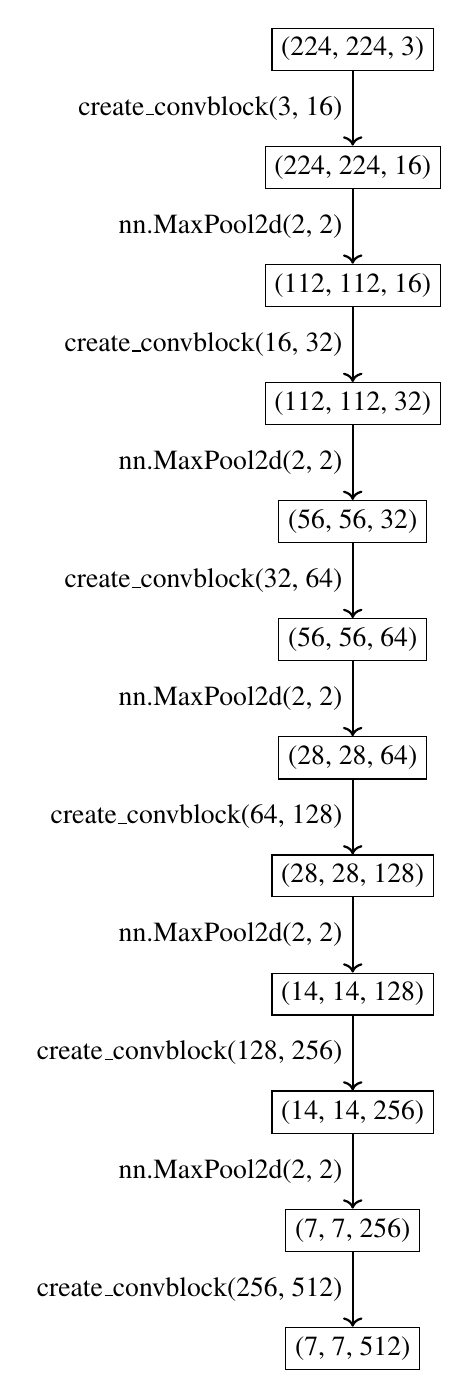
\begin{tikzpicture}
          \node[draw,  rectangle,  align=center] (box1) at (0, 0) {(224, 224, 3)};
          \node[draw,  rectangle,  align=center] (box2) at (0, -1.5cm) {(224, 224, 16)};
          \node[draw,  rectangle,  align=center] (box3) at (0, -3cm) {(112, 112, 16)};
          \node[draw,  rectangle,  align=center] (box4) at (0, -4.5cm) {(112, 112, 32)};
          \node[draw,  rectangle,  align=center] (box5) at (0, -6cm) {(56, 56, 32)};
          \node[draw,  rectangle,  align=center] (box6) at (0, -7.5cm) {(56, 56, 64)};
          \node[draw,  rectangle,  align=center] (box7) at (0, -9cm) {(28, 28, 64)};
          \node[draw,  rectangle,  align=center] (box8) at (0, -10.5cm) {(28, 28, 128)};
          \node[draw,  rectangle,  align=center] (box9) at (0, -12cm) {(14, 14, 128)};
          \node[draw,  rectangle,  align=center] (box10) at (0, -13.5cm) {(14, 14, 256)};
          \node[draw,  rectangle,  align=center] (box11) at (0, -15cm) {(7, 7, 256)};
          \node[draw,  rectangle,  align=center] (box12) at (0, -16.5cm) {(7, 7, 512)};
          \draw[->,  thick]  (box1) -- (box2) node[midway,  left] {create\_convblock(3, 16)};
          \draw[->,  thick]  (box2) -- (box3) node[midway,  left] {nn.MaxPool2d(2, 2)};
          \draw[->,  thick]  (box3) -- (box4) node[midway,  left] {create\_convblock(16, 32)};
          \draw[->,  thick]  (box4) -- (box5) node[midway,  left] {nn.MaxPool2d(2, 2)};
          \draw[->,  thick]  (box5) -- (box6) node[midway,  left] {create\_convblock(32, 64)};
          \draw[->,  thick]  (box6) -- (box7) node[midway,  left] {nn.MaxPool2d(2, 2)};
          \draw[->,  thick]  (box7) -- (box8) node[midway,  left] {create\_convblock(64, 128)};
          \draw[->,  thick]  (box8) -- (box9) node[midway,  left] {nn.MaxPool2d(2, 2)};
          \draw[->,  thick]  (box9) -- (box10) node[midway,  left] {create\_convblock(128, 256)};
          \draw[->,  thick]  (box10) -- (box11) node[midway,  left] {nn.MaxPool2d(2, 2)};
          \draw[->,  thick]  (box11) -- (box12) node[midway,  left] {create\_convblock(256, 512)};
      \end{tikzpicture}
      \caption{エンコーダの基本構造}\label{encoder}
    \end{figure}

\end{comment}
    
    \item デコード

    逆畳み込みと畳み込み作業を行う
    \begin{lstlisting}
self.Decoder = nn.Sequential(self.create_deconvblock(512, 256),  
                            self.create_convblock(256, 256), 
                            self.create_deconvblock(256, 128),  
                            self.create_convblock(128, 128), 
                            self.create_deconvblock(128, 64),  
                            self.create_convblock(64, 64), 
                            self.create_deconvblock(64, 32),   
                            self.create_convblock(32, 32), 
                            self.create_deconvblock(32, 16),  
                            self.create_convblock(16, 16), 
                            )
    \end{lstlisting}

    \verb|create_convdeblock()|では関数\verb|create_convdeblock()|が呼び出される.
    \verb|create_convblock()|では関数\verb|create_convblock()|が呼び出される.
    
    図\ref{decoder}にデコードの構造を示す.

    % \Add{コメント：縦長の図が続くので,まとめることを提案します}
    % \Add{コメント:エンコーダの最後のデータ構造とデコーダーの最初のデータ構造が異なるのは問題ないの？}
    
    \begin{figure}[H]
     \begin{minipage}[b]{0.45\linewidth}
      \centering
      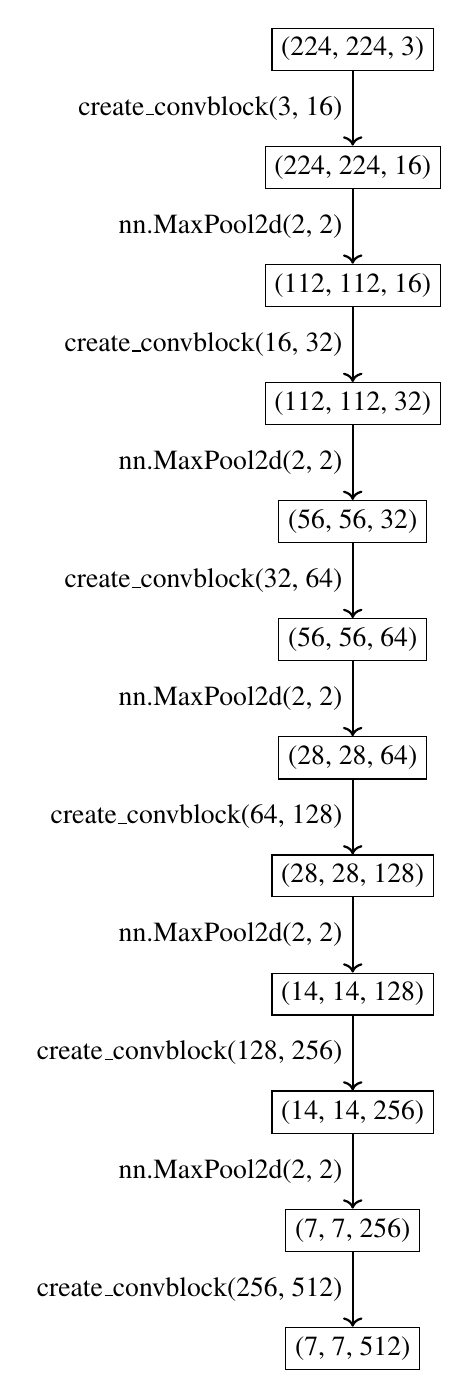
\begin{tikzpicture}
          \node[draw,  rectangle,  align=center] (box1) at (0, 0) {(224, 224, 3)};
          \node[draw,  rectangle,  align=center] (box2) at (0, -1.5cm) {(224, 224, 16)};
          \node[draw,  rectangle,  align=center] (box3) at (0, -3cm) {(112, 112, 16)};
          \node[draw,  rectangle,  align=center] (box4) at (0, -4.5cm) {(112, 112, 32)};
          \node[draw,  rectangle,  align=center] (box5) at (0, -6cm) {(56, 56, 32)};
          \node[draw,  rectangle,  align=center] (box6) at (0, -7.5cm) {(56, 56, 64)};
          \node[draw,  rectangle,  align=center] (box7) at (0, -9cm) {(28, 28, 64)};
          \node[draw,  rectangle,  align=center] (box8) at (0, -10.5cm) {(28, 28, 128)};
          \node[draw,  rectangle,  align=center] (box9) at (0, -12cm) {(14, 14, 128)};
          \node[draw,  rectangle,  align=center] (box10) at (0, -13.5cm) {(14, 14, 256)};
          \node[draw,  rectangle,  align=center] (box11) at (0, -15cm) {(7, 7, 256)};
          \node[draw,  rectangle,  align=center] (box12) at (0, -16.5cm) {(7, 7, 512)};
          \draw[->,  thick]  (box1) -- (box2) node[midway,  left] {create\_convblock(3, 16)};
          \draw[->,  thick]  (box2) -- (box3) node[midway,  left] {nn.MaxPool2d(2, 2)};
          \draw[->,  thick]  (box3) -- (box4) node[midway,  left] {create\_convblock(16, 32)};
          \draw[->,  thick]  (box4) -- (box5) node[midway,  left] {nn.MaxPool2d(2, 2)};
          \draw[->,  thick]  (box5) -- (box6) node[midway,  left] {create\_convblock(32, 64)};
          \draw[->,  thick]  (box6) -- (box7) node[midway,  left] {nn.MaxPool2d(2, 2)};
          \draw[->,  thick]  (box7) -- (box8) node[midway,  left] {create\_convblock(64, 128)};
          \draw[->,  thick]  (box8) -- (box9) node[midway,  left] {nn.MaxPool2d(2, 2)};
          \draw[->,  thick]  (box9) -- (box10) node[midway,  left] {create\_convblock(128, 256)};
          \draw[->,  thick]  (box10) -- (box11) node[midway,  left] {nn.MaxPool2d(2, 2)};
          \draw[->,  thick]  (box11) -- (box12) node[midway,  left] {create\_convblock(256, 512)};
      \end{tikzpicture}
      \caption{エンコーダの基本構造}\label{encoder}

  \end{minipage}
  \begin{minipage}[b]{0.45\linewidth}
    
      \centering
      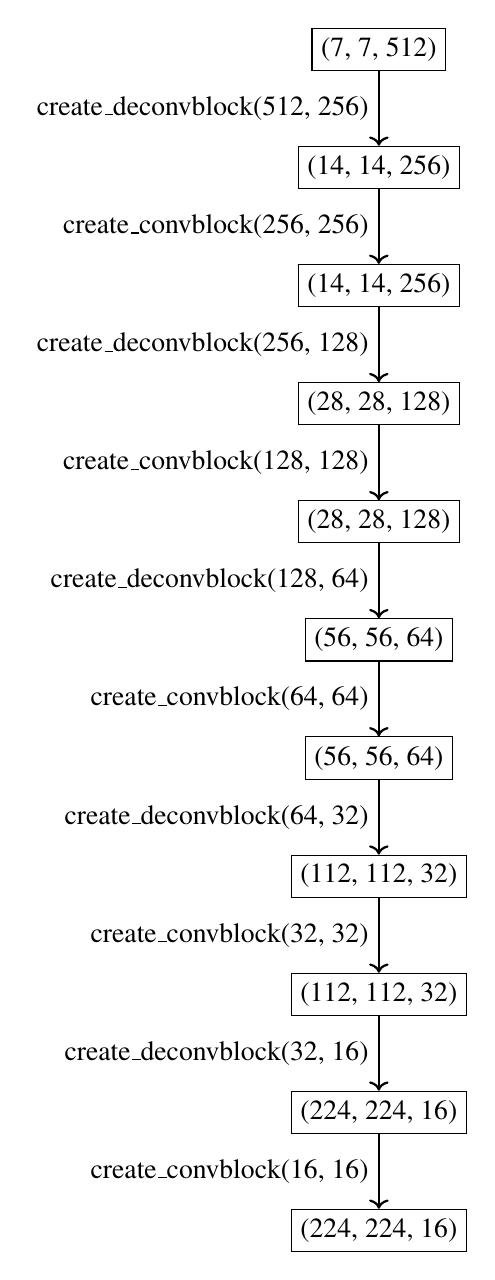
\begin{tikzpicture}
          \node[draw,  rectangle,  align=center] (box1) at (0, 0) {(7, 7, 512)};
          \node[draw,  rectangle,  align=center] (box2) at (0, -1.5cm) {(14, 14, 256)};
          \node[draw,  rectangle,  align=center] (box3) at (0, -3cm) {(14, 14, 256)};
          \node[draw,  rectangle,  align=center] (box4) at (0, -4.5cm) {(28, 28, 128)};
          \node[draw,  rectangle,  align=center] (box5) at (0, -6cm) {(28, 28, 128)};
          \node[draw,  rectangle,  align=center] (box6) at (0, -7.5cm) {(56, 56, 64)};
          \node[draw,  rectangle,  align=center] (box7) at (0, -9cm) {(56, 56, 64)};
          \node[draw,  rectangle,  align=center] (box8) at (0, -10.5cm) {(112, 112, 32)};
          \node[draw,  rectangle,  align=center] (box9) at (0, -12cm) {(112, 112, 32)};
          \node[draw,  rectangle,  align=center] (box10) at (0, -13.5cm) {(224, 224, 16)};
          \node[draw,  rectangle,  align=center] (box11) at (0, -15cm) {(224, 224, 16)};
          \draw[->,  thick]  (box1) -- (box2) node[midway,  left] {create\_deconvblock(512, 256)};
          \draw[->,  thick]  (box2) -- (box3) node[midway,  left] {create\_convblock(256, 256)};
          \draw[->,  thick]  (box3) -- (box4) node[midway,  left] {create\_deconvblock(256, 128)};
          \draw[->,  thick]  (box4) -- (box5) node[midway,  left] {create\_convblock(128, 128)};
          \draw[->,  thick]  (box5) -- (box6) node[midway,  left] {create\_deconvblock(128, 64)};
          \draw[->,  thick]  (box6) -- (box7) node[midway,  left] {create\_convblock(64, 64)};
          \draw[->,  thick]  (box7) -- (box8) node[midway,  left] {create\_deconvblock(64, 32)};
          \draw[->,  thick]  (box8) -- (box9) node[midway,  left] {create\_convblock(32, 32)};
          \draw[->,  thick]  (box9) -- (box10) node[midway,  left] {create\_deconvblock(32, 16)};
          \draw[->,  thick]  (box10) -- (box11) node[midway,  left] {create\_convblock(16, 16)};
      \end{tikzpicture}
      \caption{デコーダの基本構造}\label{decoder}

  \end{minipage}
    
    \end{figure}
    
    \item 出力前の調整
    畳み込みを行う
    \begin{lstlisting}
self.last_layer = nn.Conv2d(16, 3, 1, 1)
    \end{lstlisting}
    AutoEncoderでは最終的に画像での出力が求められているため, 
    3チャネルに戻す作業が必要である.
    図\ref{adjustment}に出力前の調整の構造を示す.
    \begin{figure}[H]
      \centering
      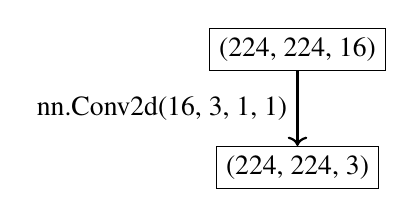
\begin{tikzpicture}
          \node[draw,  rectangle,  align=center] (box1) at (0, 0) {(224, 224, 16)};
          \node[draw,  rectangle,  align=center] (box2) at (0, -1.5cm) {(224, 224, 3)};
          
          \draw[->,  thick]  (box1) -- (box2) node[midway,  left] {nn.Conv2d(16, 3, 1, 1)};
          
      \end{tikzpicture}
      \caption{出力前の調整の基本構造}\label{adjustment}
    \end{figure}    

    \item forward関数

    AutoEncoderの実装のため, エンコード, デコードで構成される.
    また, 最終的な出力の調整用に\verb|last_layer()|も実装される.

    
    \begin{lstlisting}
def forward(self, x):
    x = self.Encoder(x)
    x = self.Decoder(x)
    x = self.last_layer(x)           
    return x
    \end{lstlisting}

    入力されたデータが$x$に代入され, \verb|__init__()|で記述したレイヤーを用いて変換が行われる.

\end{itemize}

\subsubsection{モデルの訓練}
今回畳み込みネットワークでは2重にネストされている.
外側はエポックのループ, 内側はDatasetからバッチを取り出すDataloaderによるループである.
次に, 各ループ内で以下の処理を行う.

\begin{enumerate}
    \item 勾配をゼロにする

    \item 入力をモデルに与える

    \item 損失を計算する(MSE)

    \item すべてのパラメータに対して, 損失に対する勾配を計算する

    \item オプティマイザで, 損失を減らす方向に更新する 
    
\end{enumerate}

\subsection{モデル検証}
モデル作成時に各訓練の損失を保存しているリスト\verb+loss_list["train"]+には, 訓練時の損失が格納されているため, 前節の訓練において損失が何らかの形で減少していることは確認できるが, それが十分に低いかどうかは確認することはできない.
今回の目的は入力画像と同じ画像を出力することであり, 入力画像と同じ画像が出力されたかどうかの検証は, 訓練とは独立したデータセットで確かめることが望ましい.
そこで, 先程分割した検証用データを用いてモデルを検証し, 正しく出力できたかの検証を行う.

処理内容は概ね訓練時と違いはないが, 
ネットワークをevalモードにすること(\verb|model.eval()|), パラメータの更新は行わないため, 勾配計算を不可にする処理(\verb|torch.no_grad()|)を追加する必要がある.



\subsection{訓練及び検証結果}
訓練及び検証結果としてp.\pageref{file4}の\ref{file4}「AutoEncoder学習ファイル」を実行した際の出力結果を以下に示す.
訓練を繰り返すことによって,損失(\verb|best_loss|)が減少していることが分かる.
\begin{itemize}
    \item 砂浜海岸モデル

    \begin{table}[H]
        \centering
        \begin{tabular}{|c|c|}
        
        
        
        
        
            \hline
            update best\_loss 0.042410 to 0.032781 \\
            \hline
            
            update best\_loss 0.032781 to 0.011719 \\
            \hline
            
            update best\_loss 0.011719 to 0.007017 \\
            \hline
            
            update best\_loss 0.007017 to 0.005453 \\
            \hline
            
            update best\_loss 0.005453 to 0.004682 \\
            \hline

            \vdots \\
            \hline
            
            
            
            
            
            
            update best\_loss 0.002410 to 0.002397 \\
            \hline
            
            update best\_loss 0.002397 to 0.002395 \\
            \hline
            
            update best\_loss 0.002395 to 0.002393 \\
            \hline
            
            update best\_loss 0.002393 to 0.002372 \\
            \hline
            
            update best\_loss 0.002372 to 0.002342 \\
            \hline
        \end{tabular}
        \caption{砂浜海岸モデルの学習ファイル実行結果}
        \label{makemodel1}
    \end{table}
    
    
    \item 薄いモデル

    \begin{table}[H]
        \centering
        \begin{tabular}{|c|c|}
            \hline
            update best\_loss 0.008986 to 0.008272 \\
            \hline
            
            update best\_loss 0.008272 to 0.007836 \\
            \hline
            
            update best\_loss 0.007836 to 0.007540 \\
            \hline
            
            update best\_loss 0.007540 to 0.007317 \\
            \hline
            
            update best\_loss 0.007317 to 0.007287 \\
            \hline

            \vdots \\
            \hline
            
            update best\_loss 0.004247 to 0.004224 \\
            \hline
            
            update best\_loss 0.004224 to 0.004220 \\
            \hline
            
            update best\_loss 0.004220 to 0.004209 \\
            \hline
            
            update best\_loss 0.004209 to 0.004198 \\
            \hline
            
            update best\_loss 0.004198 to 0.004190 \\
            \hline
        \end{tabular}
        \caption{薄いモデルの学習ファイル実行結果}
        \label{makemodel2}
    \end{table}

    \newpage
    
    \item 濃いモデル
    \begin{table}[H]
        \centering
        \begin{tabular}{|c|c|}
            \hline
            update best\_loss 0.009006 to 0.006873 \\
            \hline
            
            update best\_loss 0.006873 to 0.006170 \\
            \hline
            
            update best\_loss 0.006170 to 0.005986 \\
            \hline
            
            update best\_loss 0.005986 to 0.005803 \\
            \hline
            
            update best\_loss 0.005803 to 0.005422 \\
            \hline
            
            \vdots \\
            \hline
            
            update best\_loss 0.002409 to 0.002405 \\
            \hline
            
            update best\_loss 0.002405 to 0.002398 \\
            \hline
            
            update best\_loss 0.002398 to 0.002394 \\
            \hline
            
            update best\_loss 0.002394 to 0.002389 \\
            \hline
            
            update best\_loss 0.002389 to 0.002374 \\
            \hline
            
    
        \end{tabular}
        \caption{濃いモデルの学習ファイル実行結果}
        \label{makemodel3}
    \end{table}


    
    \item 周辺モデル

        \begin{table}[H]
        \centering
        \begin{tabular}{|c|c|}
        
        
        
        
        

            \hline
            update best\_loss 0.001695 to 0.000809 \\
            \hline
            
            update best\_loss 0.000809 to 0.000437 \\
            \hline
            
            update best\_loss 0.000437 to 0.000412 \\
            \hline
            
            update best\_loss 0.000412 to 0.000405 \\
            \hline
            
            update best\_loss 0.000405 to 0.000260 \\
            \hline

            \vdots \\
            \hline
            
            
            
            
            

            update best\_loss 0.000121 to 0.000120 \\
            \hline
            
            update best\_loss 0.000120 to 0.000119 \\
            \hline
            
            update best\_loss 0.000119 to 0.000119 \\
            \hline
            
            update best\_loss 0.000119 to 0.000118 \\
            \hline
            
            update best\_loss 0.000118 to 0.000117 \\
            \hline
        \end{tabular}
        \caption{周辺モデルの学習ファイル実行結果}
        \label{makemodel4}
    \end{table}
\end{itemize}
% \Add{コメント：この実行結果の数字はどのように解釈したら良いの？}

\subsection{モデルの保存とロード}

モデルが完成した場合は, モデルの保存を行う必要がある.
PyTorchでは以下のようにして, モデルをpthファイル形式で保存することができる.
\begin{lstlisting}
torch.save(model.state_dict(),  model_path)
\end{lstlisting}

今回採用したモデルの保存方法では, ファイル内にはモデル内の全てのパラメータが含まれる.
保存することができるのは重みパラメータのみでモデル構造ではないことに注意が必要である.
よって, テストや調査プログラムの使用時にはモデルのクラスを準備しておき, そのインスタンスを作って, 保存したパラメータを読み込む必要がある.

読み込みは次のようにして行うことができる.
\begin{lstlisting}
model.load_state_dict(torch.load(model_path))   
\end{lstlisting}

\subsection{差分画像の作成}
これまで説明してきた通り, テストや調査プログラムの使用時には差分画像の生成を行う.
ここでは, その手順について説明を行う.

\begin{enumerate}
    \item 画像の読み込む

    用意した画像(既に(224, 224, 3)にリサイズしたもの)を1枚ずつ読み込む
    
    \item モデルに画像を通す

    画像を通すことで, AutoEncoderで生成された画像が出力画像として生成される
    \item 差分画像の生成

    差分画像は入力画像と出力画像の差の絶対値によって求められる
    
    
\end{enumerate}
\subsection{2値画像処理の出力}
ここまでの過程でAutoEncoderを用いて, 差分画像を作成することができた.
この差分画像を用いて物体の有無を確認していく.
差分画像から物体検知の方法として2値画像処理を採用した.

今回のプログラムでは差分画像に2値化処理を行い, クロージングすることによって, より物体の輪郭を抽出しやすくした.
また, 画像内に多くの物体が観測される可能性も十分に考えられるが, 
今回検出対象とする物体は, 「ある画像に対して2値画像処理で検出された物体の中で面積が最大なもの」を採用することとした.

この理由に関しては, これまで観測された鳥の死骸の大きさのほとんどが, 分割された画像サイズに似ているものであり, 
後に人の目で判断する際に鳥の大きさ以上の物体を検出する必要があると考えたためである.
よって, 2値画像処理により, AutoEncoderで作成した差分画像から面積を算出する処理を行う.

\subsection{4つのモデルの比較}
今回, モデルを4つ作成したため, AutoEncoderで4つの差分画像, 2値画像処理で4つの面積の値が出力されることとなる.
このセクションでは4つの面積の値のどれをこの画像の物体の面積として採用するかについて説明する.

ここで2つの画像の例を用意する.
1つ目の画像の例は「物体が存在しない砂浜海岸の画像」である.
この画像をAutoEncoder並びに2値画像処理に通し, 面積を確認すると以下の結果が期待される.
\begin{itemize}
    \item 砂浜海岸モデル → この画像は既に学習済みなため, AutoEncoderを用いてうまく生成できる → 物体が検出されず面積が小さい
    \item 薄いモデル → この画像は未学習なため, AutoEncoderを用いてうまく生成できない → 物体が検出され面積が大きい
    \item 濃いモデル → この画像は未学習なため, AutoEncoderを用いてうまく生成できない → 物体が検出され面積が大きい
    \item 周辺モデル → この画像は未学習なため, AutoEncoderを用いてうまく生成できない → 物体が検出され面積が大きい
\end{itemize}
2つ目の画像の例は「物体が存在する風力発電機周辺の画像」である.
この画像をAutoEncoder並びに2値画像処理に通し, 面積を確認すると以下のようになるはずである.
\begin{itemize}
    \item 砂浜海岸モデル → この画像は未学習なため, AutoEncoderを用いてうまく生成できない → 物体が検出され面積が大きい
    \item 薄いモデル → この画像は未学習なため, AutoEncoderを用いてうまく生成できない → 物体が検出され面積が大きい
    \item 濃いモデル → この画像は未学習なため, AutoEncoderを用いてうまく生成できない → 物体が検出され面積が大きい
    \item 周辺モデル → この画像は未学習なため, AutoEncoderを用いてうまく生成できない → 物体が検出され面積が大きい
\end{itemize}

以上の例から, 1つ目のように物体がなかったとしても, その画像のバックグラウンドと異なるモデルを用いた場合, AutoEncoderでうまく画像を生成できず, 物体として出力されてしまうことが分かる.

このことからAutoEncoderを用いて1番うまく画像を生成することができたモデルの物体面積を採用すればよいと判断した. つまり
「4つのモデルの中で, 1番面積が小さいモデルの面積を採用する」ことで, 物体の有無について判断することができると言える.

\subsection{面積を用いた物体の判定基準}
これまでの説明から1枚の画像から1つの面積の値をAutoEncoderと2値画像処理を用いて求めることができた.
この面積の値を用いて物体の有無を判断することになるが, 
今回のプログラムではこの面積に上限と下限を設定し, 
この範囲内であれば, 物体有, 範囲外であれば物体無と判断することとした.

では, その上限と下限について説明していきたい.

上限は「差分画像の画素値の合計が2,400,000未満であること」である.
ここで言う差分画像の画素値の合計値とは, 面積の算出方法と同様, 4つのモデルの中で, 1番うまく生成できたモデル, つまり, 差分画像の画素値の合計が1番小さい値を言う.
この上限の役割は「濃い植生などをバックグラウンドに持つ画像の中で, 基準以上の画素値の合計値を持つ画像に関しては, 現行調査でも探索できないと判断し, 物体検出から除く」である.

実際に風力発電所見学などを通じて, 調査範囲の中には, 草木が生い茂っており, 人間の手では調査できない箇所も少なからず存在した.
それらの箇所については, ドローンでの調査においても省く必要があるため, このような上限を設定した.

下限は「面積が1,200以上であること」である.
この下限の意味は「鳥の死骸と似たような大きさの物体を検出するために, 基準以下の物体に関しては検出から除く」である.
明らかに鳥の死骸よりも小さい物体に関しては, 検出する必要がないため, このような下限を設定した.

この上限と下限は, 様々なテスト用画像を用いて, 探索した結果を十分に考慮して設定した.


\section{バードストライク調査プログラムの概要}
ここからは, 実際にバードストライク調査プログラムで使用するプログラムの流れや機能について説明する.
以下プログラムを実際に操作する人を利用者として設定する.
\subsection{事前準備}
利用者は事前準備として, ドローン画像とプログラムフォルダーの準備をする.

ドローン画像に関しては, ドローンが撮影した画像を1つのフォルダーにまとめておく.
その際そのフォルダー名は任意のもので構わない.(英小文字のみ使用可.後ほど入力する際に使用するため, 利用者はメモしておく.)
プログラムフォルダーに関しては, 特に操作は必要ない.
ドローン画像のフォルダーとプログラムフォルダーを同一階層に配置する.
\subsection{プログラムの流れ}
プログラムの大まかな流れについては以下のとおりである.
\begin{enumerate}
    \item 利用者がプログラムフォルダー内にあるexeファイル「app.exe」をダブルクリックする
    \item ドローン画像のフォルダーからファイルを読み込む
    \item ファイルを並列化処理の際に設定した分割数で分割する
    \item 画像ファイルを適切な大きさに分割する
    \item 分割した画像に対して, AutoEncoderの処理を行う
    \item 分割した画像に対して, 画像処理を行う
    \item 画像処理で算出した面積の値をもとに, 物体検出の有無を確認する.
    \item 物体有と判断した画像に対して, GUIを利用し, 利用者が鳥の死骸に該当するかどうかの判断を行う
    \item ドローン画像の中に鳥の死骸が存在した場合は, 鳥の死骸の画像およびその画像が含まれる場所を出力する
    \item ドローン画像の中に鳥の死骸が存在しなかった場合は, その旨を出力する
\end{enumerate}
\subsection{プログラム機能}
\subsubsection{スタート画面}
\begin{figure}[H]
    \centering
    \includegraphics[width=1\linewidth]{s1.png}
    \caption{スタート画面}
    \label{s1}
\end{figure}
プログラムの実行がされた際に, 初めにプログラムでは以上の画面が表示される.
この画面では, 主にドローン画像が格納してあるフォルダー名とプログラムを実行する際の注意点について記載する.
GUIのEntryウィジェットを用いて, 利用者にフォルダー名を入力させ, フォルダー名を取得する.

注意事項として, プログラム内で音声を使用するため, PC等の音量の調整をすること, 
GUIが表示されるウィンドウの「×ボタン」を押して終了せず, GUI内にあるボタンを押して終了することが記載してある.
入力と確認が終了すれば, 「確認ボタン」を押す.


\subsubsection{エラー画面}
\begin{figure}[H]
    \centering
    \includegraphics[width=1\linewidth]{s2.png}
    \caption{エラー画面}
    \label{s2}
\end{figure}
この画面は, 入力に応じて取得したフォルダー名を基に, ドローン画像が格納してあるフォルダーを探したが, 見つからなかった旨を知らせる画面である.
見つからなかった理由としては, フォルダー名を誤って入力した,画像フォルダーとプログラムフォルダーが同一階層に配置されていないなどが考えられる.
この画面は数秒後自動的に閉じられ, プログラムも同時に終了する.
この画面が出た利用者はフォルダー名やフォルダーの場所が適切かどうか再度確認し, プログラムの再実行が必要である.


\subsubsection{実行待機画面}
\begin{figure}[H]
    \centering
    \includegraphics[width=1\linewidth]{s8.png}
    \caption{実行待機画面}
    \label{s8}
\end{figure}
この画面は, AutoEncoder処理並びに画像処理の実行時に画面上に表示されるものである.
この画面の持つ意味は, 利用者に処理が実行中であることを知らせる, PC等でほかの処理をしないようにする, などがある.
実行が終了すれば, この画面は自動で閉じられる.


\subsubsection{実行終了画面}
\begin{figure}[H]
    \centering
    \includegraphics[width=1\linewidth]{s9.png}
    \caption{実行終了画面}
    \label{s9}
\end{figure}
この画面では, AutoEncoder処理並びに画像処理の実行が終了したことを知らせる.
この画面の表示とともに, 音声が数秒間鳴り, 利用者に実行終了をアナウンスする.
画像の枚数が増えれば増えるほど, 実行時間は長くなるため, 
音声で知らせることで, 実行中も他の作業や別の風力発電機への移動などをすることができる.
利用者は確認することができた場合, 画面下部の「確認ボタン」を押し, 次の作業に移る.



\subsubsection{判定準備画面}
\begin{figure}[H]
    \centering
    \includegraphics[width=1\linewidth]{s3.png}
    \caption{判定準備画面}
    \label{s3}
\end{figure}

この画面では, これから利用者が行う判定作業に関して, やり方や注意事項を記載している.
具体的には, 表示される全ての画像に対して, 鳥の死骸に該当するかしないかの判断作業を利用者に説明する.
利用者は確認後「確認ボタン」を押すことで, この画面は閉じられる.


\subsubsection{判定画面}
\begin{figure}[H]
    \centering
    \includegraphics[width=1\linewidth]{s10.png}
    \caption{判定画面}
    \label{s4}
\end{figure}

この画面では, 利用者に判定作業を行ってもらう.
図\ref{s4}はテスト用画像(p.\pageref{2023年5月30日撮影画像},図\ref{2023年5月30日撮影画像})を使用し
実際の判定作業のイメージを掲載したものである.

具体的な内容としては, 鳥の死骸だと考える場所をクリックする.
クリックした場所は赤く表示され, それと同時にコンピュータにはその場所の座標が記憶される.
クリックした場所を修正したいときには, 再度クリックすると元の状態に戻る.
画像の枚数が画面に表示される画像の数より少なければ, その場所は白く表示される.
利用者は判定作業が終了すれば, キーボードの「Enterキー」を押すと, 画面が閉じられる.
% \Add{コメント:「クリックした場所は赤く表示」は図18に現れていない？}


\subsubsection{再調査画面}
\begin{figure}[H]
    \centering
    \includegraphics[width=1\linewidth]{s5.png}
    \caption{再調査画面}
    \label{s5}
\end{figure}

この画面では, 利用者に判定作業の再調査は必要かどうかを確認する.
利用者が判定作業にミスがあったと判断した場合, 画面右下の「再調査ボタン」を押すことで, 再度判定作業をすることができる.
具体的には, 「再調査ボタン」が押された場合, これまでの判定結果を破棄し, 判定画面を表示するプログラムまで戻る.
画面左下の「調査終了ボタン」を押すと, 調査は終了し, 画面は閉じられる.


\subsubsection{鳥発見無画面}
\begin{figure}[H]
    \centering
    \includegraphics[width=1\linewidth]{s6.png}
    \caption{鳥発見無画面}
    \label{s6}
\end{figure}

この画面では, 鳥の死骸が発見されなかったときにその旨を知らせる.
具体的には, 判定作業で利用者が累計で画像を1枚もクリックしなかったときに表示される画面である.
数秒後画面は自動的に閉じられ, 同時にプログラムも終了する.


\subsubsection{鳥発見有画面}
\begin{figure}[H]
    \centering
    \includegraphics[width=1\linewidth]{s7.png}
    \caption{鳥発見有画面}
    \label{s7}
\end{figure}

この画面では, 鳥の死骸が発見された旨と鳥の死骸が保存してあるフォルダー名を知らせる.
具体的には, 判定作業で利用者が通算で画像を1枚以上クリックしたときに表示される画面である.
また, 保存された鳥の死骸の画像は「「bird\_image」+「プログラムの開始時間の文字列」」の名前のフォルダーに, 
ドローン画像フォルダーやプログラムフォルダーと同一階層に保存されている.
画像のフォルダー名で座標情報が確認できる.
数秒後画面は自動的に閉じられ, 同時にプログラムも終了する.
% \Add{死骸が移っていた写真の座標情報はどこに残されているの？}

\section{結論}
バードストライク調査プログラムの評価として, プログラム内の物体判定基準に基づき, 
「プログラムが物体を検出したか否か」についてテストデータを用いて評価する.

\subsubsection{評価方法}
今回のバードストライク調査の場合において, 
物体が存在するケースをTrue, 物体が存在しないケースをFalseとすると, 
混合行列のそれぞれの要素は以下のようになる.
\begin{itemize}
    \item True Positive(TP)

    モデルが物体が存在すると分類したとき, 実際に物体が存在する画像
    
    \item False Positive(FP)

    モデルが物体が存在すると分類したとき, 実際には物体が存在しない画像
    \item False Negative(FN)

    モデルが物体が存在しないと分類したとき, 実際には物体が存在する画像
    \item True Negative(TN)

    モデルが物体が存在しないと分類したとき, 実際に物体が存在しない画像
\end{itemize}

次にこの調査のタスクを整理すると以下になる.

\begin{itemize}
    \item 物体が存在する画像を物体が存在しないと分類することはNG(FNはNG).
    \item FPは許容するが, 少なくしたい.
\end{itemize}

また, データセットの大まかな特徴は以下である.
\begin{itemize}
    \item 物体が存在する画像よりも物体が存在しない画像が多い不均衡データである.
\end{itemize}

以上を踏まえて, 評価指標を検討すると, 以下となる.


\begin{table}[H]
    \centering
    \begin{tabular}{|c|p{12cm}|}
        \hline
        \textbf{評価指標} & \multicolumn{1}{c|}{\textbf{検討内容}}\\
        \hline 
        
        正解率 & 扱うデータが不均衡であるため使用しないほうがよい\\
        \hline
        
        MCC & 混合行列の要素によって重要度に違いがあるため使用しないほうがよい\\
        \hline
        
        適合率 & 「FPは許容するが, 少なくしたい」の条件に対応できる指標である\\
        \hline
        
        再現率 & 「物体が存在する画像を物体が存在しないと分類することはNG(FNはNG)」の条件に対応できる指標である\\
        \hline
        
        F1-socre & FPよりもFNの評価が高いため, 工夫が必要である\\
        \hline

        G-Mean & Negativeの予測漏れは許容できるがPositiveの予測漏れは許容できないため, 使用しないほうがよい\\
        \hline
        
    \end{tabular}
    \caption{評価指標の検討結果}
    \label{cost}
\end{table}

以上のことから, 今回評価指標としては, 
$F_{\beta}-score$を${\beta}=2$として「適合率」を重視した$F_{2}-score$を採用する.
また, サブ評価として適合率と再現率も同時に算出する.

\subsubsection{評価結果}
今回は,より実際の調査と近い環境での評価を行うため, 学習に使用した画像ではなく, 全く別の日に撮影した画像を用いた.
この画像は2023年5月30日にドローンで上空15mから撮影から撮影した物であり, 画像のサイズは3000×4000である.
縮小した画像を図\ref{2023年5月30日撮影画像}に示す.

\begin{figure}[H]
    \centering
    \includegraphics[width=1\linewidth]{20230530_15.JPG}
    \caption{撮影画像}
    \label{2023年5月30日撮影画像}
\end{figure}

初めに画像の分割を行う.
画像を224×224の大きさに分割するため, 用意した画像から221枚の画像が生成される.
この221枚の画像に対して, 学習と同様に反転と回転を行ってできた全3536枚が用意できた.

次に手作業によって「物体有の画像」と「物体無の画像」に分割する.
「物体有の画像」と判断したのは3536枚中96枚, 「物体無の画像」と判断したのは3536枚中3440枚であった.

次にプログラムを使用しての物体検出を行う.
プログラムの物体検出は, \ref{mainfile}「プログラムメインファイル」のautoencoder関数に記載している.

物体検出の結果を表\ref{matrix}の混合行列を用いて示す.

\begin{table}[H]
    \centering
    \begin{tabular}{|cc|c|c|}
        \cline{3-4}
        \multicolumn{2}{c|}{} & \multicolumn{2}{c|}{モデルによる分類結果(予測)}\\
        \cline{3-4}
        \multicolumn{2}{c|}{} & 物体有(194枚) & 物体無(3342枚) \\ 
        \hline
        \multirow{2}{*}{真のクラス(正解)} & \multicolumn{1}{|c|}{物体有(96枚)} & TP(96枚) & FN(0枚) \\
        \cline{2-4}
         & \multicolumn{1}{|c|}{物体無(3440枚)} & FP(98枚) & TN(3342枚)\\ \hline
    \end{tabular}
    \caption{混合行列}
    \label{matrix}
\end{table}

以上の結果からF2-score, 適合率, 再現率を算出する.
\begin{itemize}
    
    \item 適合率

    \begin{equation}
        適合率(Precision) = \frac{TP}{TP+FP} = \frac{96}{96+98} = 0.49
    \end{equation}
    \item 再現率

    \begin{equation}
        再現率(Recall) = \frac{TP}{FN+TP} = \frac{96}{96+0} = 1.00
    \end{equation}
    \item F2-score

    \begin{equation}
        F_{2} = \frac{5 \times 再現率 \times 適合率}{(4 \times 適合率)+再現率} = 
        \frac{5 \times 1.00 \times 0.49}{(4 \times 0.49)+1.00} = 0.83
    \end{equation}
\end{itemize}


\subsubsection{課題と展望}
今回のバードストライク調査プログラムにおいて, このプログラムを使用することで高い精度で物体を検出することができた.
これにより, 調査員が確認する画像は図22の画像において3536枚から194枚と大幅に削減することができた.
また, 確認作業によって本来の目的である鳥の死骸の発見を達成することが可能である.
このプログラムの実行時間は風力発電機1基当たり30分未満であることが確認されており, ドローンの飛行時間が約30分であることを考えると, 調査の省力化並びに時間削減に成功したと言える.

今後の課題としては以下の2つ挙げられる.

1つ目は対応可能な撮影条件を増やすことである.
p.\pageref{feedback}の\ref{feedback}「月例報告会」からも指摘があった通り, 例として積雪が確認された日の調査の場合, モデルの学習には雪のバックグラウンドを学習していないため, 物体検出の精度は良くないと想定される.
また, 今後別の植生や風力発電機の調査を行う場合, モデルの構造やパラメータ変更の必要が生じる可能性がある.

2つ目は鳥の死骸発見までを自動化することである.
実際には調査員の業務としてバードストライク調査だけではなく, 風力発電機の点検や発電機周囲の異常確認等, 業務は多数存在する.
現状では自動的に行うことができるのは, 物体の検出までであり, このプログラムではプログラムの実行時間の他に, 調査員の判定作業時間が別に必要であり, 実際にはバードストライク調査に30分以上の時間が必要である.

今後とも研究室ではバードストライク調査の研究を続けていき, 最終的な目標としては, 判定作業をなくし, 鳥の死骸検出までを全自動で行うことである.この目標が達成できれば, 判定作業分の時間で他の業務をすることが可能で, さらに省力化や時間削減につながる.具体的な案としては, 物体が検出された画像のみを学習し, 「鳥の死骸の画像」と「鳥の死骸ではない画像」に分類することで, 「鳥の死骸の画像」のみを検出することができるのではないかと考える.


\subsubsection{月例報告会から}\label{feedback}
本研究ではプログラム作成に当たり, 実際に調査を行う山形県企業局酒田電気水道事務所との月例報告会を毎月を行っていた.
月例報告会では主にプログラムの機能面について, 研究室から改善内容を報告し, 事務所から要望並びに意見をいただいた.
今年度最後の月例報告会となった2023年12月13日には事務所からこのプログラムの総評としてご意見を頂戴したため, その一部を記載する.

\begin{itemize}
    \item 事務所側から要望した内容が十分に反映・改良されていた

    \item 物体が検出された画像に関しては, 元の画像も出力してほしい

    \item 判定作業の際に, 画像を拡大・縮小作業ができればありがたい

    \item 拡大・縮小機能ができなければ, 表示画像枚数を少なくすることも考える必要がある

    \item 冬の時期に積雪が確認できる状況で調査を行う可能性があるため,バックグラウンドが積雪の状態の画像は学習していないが, 調査は可能か
    
\end{itemize}


\section{謝辞}
本研究をまとめるにあたり, 多くの方々にご助力いただきましたこと, 心より感謝申し上げます.指導教官として豊富な知識と経験の下, 適切な助言と終始多大なご指導を賜りました山形大学大学院理工学研究科脇克志教授に深く感謝いたしますとともに, 御礼申し上げます.約3年間の間, 研究活動に携わらせていただいた中で, 興味を持っていた画像処理と深層学習について学ぶことができ, 非常に大きな力となりました.また, 学会等に参加させていただいたことは, 自分自身の価値観を広げる貴重な経験となりました.

次に, 副指導教員として深層学習およびPythonに関する様々な知識とご助言を賜りました, 山形大学理工学研究科Yago Diez准教授に厚くお礼申し上げます.モデルの作成や仕組みについて深く学ばせていただき, 多くのご指導を賜りました.

さらに, 研究に関しての画像提供をはじめとする研究協力をいただきました, 山形県企業局酒田電気水道事務所(平田浄水場)渡邊弘章様, 齋藤洋美様, 村上浩様, 木村俊之様, 大友浩一様, 荒井隆男様, 鈴木旺様に深く感謝申し上げます.風力発電所での調査見学や月例報告会でも多くのご意見をいただき, 非常に感謝しております.

また, 同じ研究室のゼミ生として, 切磋琢磨しながら研究活動を行ってきた, 森竹孝磨さん, 千葉歩夢さんに厚くお礼申し上げます.お二人と一緒に活動できたおかげで, 自分自身も楽しく活動しながらも成長することができました.

最後になりますが, 大学生活において自分に携わってくださった全ての皆様,  これまで自分を育ててくれた両親に感謝いたします.
\section{参考文献}
% 参考文献を作るための参考文献：http://www.ic.daito.ac.jp/~mizutani/tex/drill/drillbook3.html
% https://www.rakuten-card.co.jp/minna-money/topic/article_2305_00063/
\begin{thebibliography}{99}
    \bibitem{参照ラベル名1} チーム・カルボ. 物体検出とGAN, オートエンコーダー, 画像処理入門 PyTorch/TensorFlow2による発展的・実装深層学習. 1版, 株式会社 秀和システム, 2021, 459p
    \bibitem{参照ラベル名2} 小枝正直・上田悦子・中村恭之. OpenCVによる画像処理入門 改定第2版. 2版, 株式会社 講談社, 2017, 256p
    \bibitem{参照ラベル名3} Eli Stevens・Luca Antiga・Thomas Viehmann. Pytorch実践入門 深層学習の基礎から実装へ. 1版, 株式会社 マイナビ出版, 2021, 591p
    \bibitem{参照ラベル名4} 八谷大岳. 機械学習スタートアップシリーズ ゼロからつくるPython機械学習プログラミング入門. 1版, 株式会社 講談社, 2020, 349p
    \bibitem{参照ラベル名5} 高木章光/鈴木英太. 図解入門 最新 データサイエンスがよ～くわかる本. 1版, 株式会社 秀和システム, 2019, 263p
    \bibitem{参照ラベル名6} 増井敏克. 図解まるわかり データサイエンスのしくみ. 1版, 株式会社 翔泳社, 2022, 239p
    \bibitem{参照ラベル名7} Ankur A. Patel. Pythonではじめる教師なし学習 -機械学習の可能性を広げるラベルなしデータの利用. 1版, 株式会社 オライリー・ジャパン, 2020, 317p
    \bibitem{参照ラベル名8} 我妻幸長. はじめての深層学習. 1版, SBクリエイティブ株式会社, 2018, 322p
    \bibitem{参照ラベル名9} 我妻幸長. はじめての深層学習2. 1版, SBクリエイティブ株式会社, 2020, 330p
    \bibitem{参照ラベル名10} 小畑正貴. たのしくできる 並列処理コンピュータ. 1版, 東京電機大学出版所, 2001, 197p
    \bibitem{参照ラベル名11} 高柳慎一, 長田怜士. 評価指標入門~データサイエンスとビジネスをつなぐ架け橋~. 1版, 株式会社技術評論社, 2023, 261p
    \bibitem{参照ラベル名12} 吉村康弘, 杉浦司, 五木田和也. OpenCVではじめよう深層学習による画像認識. 1版, 株式会社技術評論社, 2022, 297p

    \bibitem{参照ラベル名13} Francois Chollet. PythonとKerasによる深層学習. 1版, 株式会社マイナビ出版, 2018, 376p
    \bibitem{参照ラベル名14} Aurelien Geron. scikit-learn, Keras, TensorFlowによる実践機械学習 第2版. 2版, 株式会社オライリー・ジャパン, 2020, 798p
    \bibitem{参照ラベル名15} 浦達也.  "風力発電が鳥類に与える影響 -環境紛争・規模・立地の観点から-". 第1回 再生可能エネルギーの適正な導入に向けた環境影響評価のあり方に関する検討会.\url{https://www.meti.go.jp/shingikai/safety_security/renewable_energy/pdf/001_03_04.pdf}. (参照 2024-01-23)
    \bibitem{参照ラベル名16} 自然エネルギー庁. "事業計画策定ガイドライン". 2023. \url{https://www.enecho.meti.go.jp/category/saving_and_new/saiene/kaitori/dl/fit_2017/legal/guideline_wind.pdf}. (参照 2024-01-23)
    \bibitem{参照ラベル名17} 経済産業省 自然エネルギー庁.  "再生可能エネルギー 固定価格買取制度ガイドブック2018年度版". 2018. \url{https://www.enecho.meti.go.jp/category/saving_and_new/saiene/data/kaitori/2018_fit.pdf}. (参照 2024-01-23)
    \bibitem{参照ラベル名18} 環境省地球温暖化対策課.  "概要資料導入編". 我が国の再生可能エネルギー導入ポテンシャル. 2022. \url{https://www.renewable-energy-potential.env.go.jp/RenewableEnergy/doc/gaiyou3.pdf}. (参照 2024-01-23)
    \bibitem{参照ラベル名19} 経済産業省 自然エネルギー庁.  "再生可能エネルギーとは". なっとく！再生可能エネルギー. \url{https://www.enecho.meti.go.jp/category/saving_and_new/saiene/renewable/wind/index.html}. (参照 2024-01-23)
    \bibitem{参照ラベル名20} 佐藤岳.  "山形県エネルギー戦略に基づく取り組みについて". 特集 風力発電尾地域導入への取り組みと社会受容性の向上, 並び日に地域振興を目指して. 
    \url{https://www.jstage.jst.go.jp/article/jwea/38/1/38_73/_pdf/-char/ja}. (参照 2024-01-23)
    \bibitem{参照ラベル名21} 浦達也.  "風力発電が鳥類に与える影響の国内事例".  2015. \url{https://www.wbsj.org/nature/public/strix/31/strix31_03.pdf}. (参照 2024-01-23)
    \bibitem{参照ラベル名22} Makoto Hiroi.  "新・お気楽 Python/Tkinter 入門".  2006. \url{http://www.nct9.ne.jp/m_hiroi/light/pytk01.html}. (参照 2024-01-23)
    \bibitem{参照ラベル名23}kdl-di. 【やってみた】 "AutoEncoder+MVTecデータセットで異常検知". 神戸のデータ活用塾!KDL Data Blog. 2022. \url{https://kdl-di.hatenablog.com/entry/2022/04/28/090000}. (参照 2024-01-24)
\end{thebibliography}

\section{付録}
\subsection{プログラムメインファイル}
\begin{lstlisting}
import time
import datetime
import glob
import re
import cv2
import threading
import numpy as np
import datetime
import os
import pygame
import tkinter as tk
from AE_production_GUI_complete import GUI_start,  GUI_error,  GUI_judge,  GUI_again,  GUI_nobird,  GUI_bird,  GUI_judge_start
from AE_production_testmodel_complete import AE,  make_models

# 使用するモデルの作成
# 使用するモデルのパス(変更可)
model_paths = ["AEmodel_dark_green20231223.pth",  "AEmodel_light_green20231223.pth",  "AEmodel_paved_ground20231223.pth",  "AEmodel_white20231223.pth"]
models = make_models(model_paths)

# 並列化分割数
number_of_threads = 8
# 閾値の上限
area_threshold = 1200

# 日付を取得する
t_delta = datetime.timedelta(hours=9)
JST = datetime.timezone(t_delta,  'JST')
now = datetime.datetime.now(JST)
Datetime = '{:%Y%m%d%H%M%S}'.format(now)

# フォルダーの名前をGUIを使って入力
folder_name = GUI_start()
# フォルダーがデスクトップになければエラーを出力する
if not os.path.isdir(folder_name):
    GUI_error()
    exit()

# 読み込み開始
def atoi(text):
    return int(text) if text.isdigit() else text

def natural_keys(text):
    return [ atoi(c) for c in re.split(r'(\d+)',  text) ]

files = sorted(glob.glob(f"{folder_name}/*"),  key=natural_keys)
# 読み込み完了

# 画像分割サイズ
distance = 224

# 画像判定用白色画像
red_image = np.zeros((distance,  distance,  3),  np.uint8)+255

# マルチスレッド開始
# スレッド数でフォルダーを分割
# 商
quotient = len(files) // number_of_threads
# 余り  
remainder = len(files) % number_of_threads

# 余り以外のファイル名を分割して１つのリストにする
filelists = [files[quotient * i:quotient * (i + 1)] for i in range(number_of_threads)]
# 余りのファイル名のリストを作成
quot_list = files[quotient * number_of_threads:quotient * number_of_threads + remainder]
# 合体させて１つのリストにする
filelists.append(quot_list)

# 画像を分割する関数
def split(FILES):
    # 分割後の画像を分割前の画像ごとに格納
    split_images = []
    for i in range(len(FILES)):
        file = FILES[i] #ファイル名
        img = cv2.imread(file) #画像読み込み
        h,  w = img.shape[:2] #画像のサイズ
        # 分割の始点
        cx = 0 
        cy = 0
        for x in range(h//distance):
            for y in range(w//distance):
                # 画像の切り取り
                split_img = img[cx:cx+distance,  cy:cy+distance]
                # 画像の格納
                split_images.append(split_img)
                cy += distance
            cy = 0
            cx += distance
    return split_images

# AutoEncoderに通す関数
def autoencoder(IMAGES,  models):
    # AEに通した結果を保存しておくリスト(鳥がいるかいないか)
    AE_judge_result = []
    # AEに通した結果の画像を保存しておくリスト
    AE_image_result = []
    # 画像は1枚ずつ
    for idx,  image in enumerate(IMAGES):
        # 呼び出した関数からは面積と輪郭画像が出力されてくる
        area = AE(image,  models)
        # 画像はどちらにしても保存
        AE_image_result.append(image)

        # 面積がしきい値より小さければ, 鳥なしとして格納
        if area < area_threshold:
            AE_judge_result.append(False)
        # 面積がしきい値より大きければ, 暫定鳥ありとして格納
        else:
            AE_judge_result.append(True)
        
    return AE_judge_result,  AE_image_result


# メインの処理を行う関数
def split_and_autoencoder(fl,  al,  ai):
    # 画像を分割
    images = split(fl)
    # AutoEncoderに通して, 判定結果を保存
    judge_list,  images_list = autoencoder(images,   models)
    al += judge_list
    # AutoEncoderに通して, 結果画像を保存
    ai += images_list
    return

# スタート時間
time_start = time.time()

# スレッドを格納するリスト
threads = []
# 判定結果を格納するリスト
autoencoder_list = []
# 結果画像を格納するリスト
autoencoder_image = []
# AutoEncoder実行中のGUI
# GUIの画面
root = tk.Tk()
# GUIのタイトル
root.title("実行中です")
# GUIを全画面表示にする
root.state("zoom")
# GUIに表示するコメントのフォント設定
font1 = tk.font.Font(family='Helvetica',  size=100,  weight='bold')
# GUIに実行中の旨のコメントを表示
label = tk.Label(root,  text="実行中です\nしばらくお待ちください\n実行が終了しましたら\n音声でお伝えします",  font=font1)
# コメントの配置
label.pack(anchor='center', expand=1)
# スレッドが完遂しているかどうかのチェック関数
def check_threads():
    # スレッドを１つ１つ確認し, 完了しているかどうかチェック
    for th in threads:
        # 未完了のスレッドがあれば, コメント表示を続ける
        # １０秒ごとにスレッドの終了確認をする
        if th.is_alive():
            root.after(10000,  check_threads)
            return
    # スレッドが終了していたら, 音楽を鳴らす
    # 音楽(mp3ファイル)の読み込み 
    mp3_path = "decide21.mp3"
    # 作業が終了したというコメントの変更
    label.config(text="作業が終了しました")
    # 音楽を鳴らすための関数
    def play_mp3(mp3_path):  
        pygame.mixer.init()
        pygame.mixer.music.load(mp3_path)  
        pygame.mixer.music.play()
    # GUIを終了させる関数
    def finish():
        root.destroy()
        return
    # 確認ボタン
    button = tk.Button(root,  text = '確認',  command=finish,  bg='#f0e68c',  height=5,  width=20)
    # ボタンの設置
    button.pack(side = tk.BOTTOM)
    # 音楽を鳴らす関数の実行
    play_mp3(mp3_path)

for filelist in filelists:
    #マルチスレッド用の画像読み込み関数（imread_worker）のスレッドを立てる
    t = threading.Thread(target=split_and_autoencoder,  args=(filelist,  autoencoder_list,  autoencoder_image),  daemon=True)
    #スレッドの開始
    t.start()
    #スレッドリストへ格納
    threads.append(t)

#全てのスレッドが終わるまで待つ
root.after(10000,  check_threads)
root.mainloop()

# GUIでの判定を行う関数
def bird_judge(judge_list,  image_list):
    # GUIでの判定が必要な画像
    judge_image = []
    # 必要な画像のインデックス
    idx_image = []
    # 全ての画像に対して, AEが物体検出をすればGUIでの判定が必要
    for idx,  judge in enumerate(judge_list):
        if judge:
            judge_image.append(image_list[idx])
            idx_image.append(idx)
    if len(judge_image) == 0:
        return [],  []
    # 画像を144枚ずつGUIで表示するが, 余った画像は赤色画像を補填
    judge_image += [red_image for _ in range(144-len(judge_image)%144)]
    # GUIが鳥ありと判断した画像を保存
    bird_image = []
    # 鳥ありと判断した画像の通し番号
    bird_image_number = []
    # 判定必要な全ての画像に対して, GUIでの判定を行う
    for i in range(len(judge_image)//144):
        # 画像を144枚ごとに区切る
        images = judge_image[144*i:144*(i+1)]
        # 画像をタイル状に並べる(9×16)
        image = [[] for _ in range(9)]
        for j in range(144):
            image[j//16].append(images[j])
        judge_set = GUI_judge(image)
        for J in judge_set:
            bird_image.append(images[J])
            bird_image_number.append(idx_image[144*i+J])
    
    return bird_image,  bird_image_number

# 時間計測
time_end = time.time()
TIME = int(time_end-time_start)
print("-------------実行情報-------------")
print("ドローン画像の枚数",  len(files),  "枚")
print("分割後の画像総枚数",  len(autoencoder_list),  "枚")
print("物体検出枚数",  autoencoder_list.count(True),  "枚")
print("実行時間(ユーザーの操作外)",  TIME//60,  "分",  TIME%60,  "秒")
print("----------------------------------")

# 判定作業開始画面
GUI_judge_start()
# もし, 操作違いなどでもう一度やり直したい場合への対応
while True:
    # GUIでの判定作業を行う
    bird_image,  bird_image_number = bird_judge(autoencoder_list,  autoencoder_image)
    # GUIで判定を終了してよいか確認し, 了承を得たら終了する
    if not GUI_again():
        break

one_image_number = len(autoencoder_list)//len(files)
# 鳥の画像が0枚だったら, 鳥がいないと判断し終了する
if len(bird_image) == 0:
    GUI_nobird()
# 鳥がいたら, デスクトップにフォルダーを作成し, その中に鳥の画像を保存する
else:
    os.makedirs(f"../bird_image{Datetime}")
    i = 0
    for idx in bird_image_number:
        cv2.imwrite(f"../bird_image{Datetime}/image{idx//one_image_number+1}-{i}.jpg",  bird_image[i])
        i += 1
    GUI_bird(Datetime)
}
\end{lstlisting}\label{mainfile}

\subsection{グラフィカルユーザーインターフェース(GUI)}
% http://www.nct9.ne.jp/m_hiroi/light/pytk01.html
% \Add{このGUIの記述は,Tkinterの一般的な説明だけなので,付録の最初として8.1に移動した方が良い}
バードストライク調査プログラムでは, プログラム内の画面表示としてGUIを使用した.
このセクションではPythonでGUIを作成するためのライブラリであるTkinterを使用したGUIの作成方法を説明する.

\subsubsection{event駆動方式}
GUIアプリケーションの場合, ユーザーからの入力やシステムの状態変化など, ある出来事をきっかけにプログラムが実行される.
この出来事を\textbf{event}といい, eventをきっかけにしてプログラムが起動されることを\textbf{eventdriven}という.
eventdriven型のアプリケーションは, 一般に以下の1.の初期化を実行した後に2と3を交互に繰り返す.
\begin{enumerate}
    \item 初期化
    \item eventの取得
    \item eventの種類に応じて処理を振り分ける
\end{enumerate}

この交互の繰り返しをeventループと呼び, アプリケーションはユーザーからの入力などのeventを待つ.
そして, 3の処理に対応する機能が\textbf{binding}である.
bindingは, ウィンドウでeventが発生したときに, それに応じて定義したプログラムを実行する.
このプログラムをeventハンドラやコールバック関数と呼ぶ.
% \Add{コメント：「event」と「event」が混在しているどちらか1つに統一する}

\subsubsection{Tkinterで必要な手順}

TkinterでGUIアプリケーションを作る場合, 次のような手順が必要になる.
\begin{enumerate}
    \item トップレベルのウィンドウ(メインウィンドウ)を作る
    \item ウィジェット(部品)を設定してウィンドウに配置する
    \item eventループを開始してユーザーからの要求(event)を処理する
\end{enumerate}

この他に必要に応じてコールバック関数を作成する.
次に, 実際にプログラムを見ながらGUIアプリケーションについて解説する.
例として, ボタンを1つ作成するプログラムを以下に示す.

\begin{lstlisting}
import tkinter as tk

root = tk.Tk()
root.option_add('*font',  ('Noto Sans CJK JP',  10))

button = tk.Button(root,  text = 'Hello,  Python/Tkinter')
button.pack()

root.mainloop()
\end{lstlisting}

また,このプログラムを実行した結果のウィンドウを以下に示す.
\begin{figure}[H]
    \centering
    \includegraphics[width=0.5\linewidth]{button.PNG}
    \caption{ボタンのGUIアプリケーション}
    \label{button}
\end{figure}

初めに, \verb+Tk()+でメインウィンドウを作成する.
Tkinterはオブジェクト指向を使って作られており, \verb|Tk()|はクラス\verb+Tk+のインスタンス(オブジェクト)を生成して返す.
このオブジェクトが画面上のメインウィンドウに対応する.

次にボタンを作成する.
 \verb|Tk()|ではGUI用の部品のことをウィジェットと呼ぶ.
 \verb|Tk()|は多くのウィジェットが用意されており, それをウィンドウに配置することで簡単にGUIアプリケーションを作成することができる.
Tkinterの場合, ウィジェット名と同じクラスが用意されており, ボタンを作るには\verb|Button()|でボタンのオブジェクトを生成する.
この時, 第1引数にウィジェットを配置するウィンドウのオブジェクトを渡す.
引数 \verb+text = 'Hello,  Python/Tkinter'+はボタンに表示されるテキストを指定する.

この段階ではボタンはまだ配置されておらず, ボタンの配置はメソッド\verb|pack()|で行う.
Tkの場合, ウィジェットの配置はジオメトリマネージャが行う.
3種類のマネージャが存在し, \verb|pack()|はそのうちの1つである.
\verb|button.pack()|が実行されるとウィンドウにボタンが配置される.
最後に\verb|mainloop()|を呼び出して, eventループを開始する.

これは簡単なプログラムだが, TkinterでGUIアプリケーションを作る場合の基本的な構造を表している.
このプログラムではボタンを表示しただけであるが, コールバック関数では押したときの動作のプログラムを設定することができる.

\subsubsection{ウィジェットの種類}

Tkinterが保持する主なウィジェットについてを表\ref{Tk}に示す.
\begin{table}[H]
    \centering
    \begin{tabular}{|c|c|c|}
    \hline
    \textbf{ウィジェット名} & \textbf{クラス名	}  & \multicolumn{1}{c|}{\textbf{概要}} \\
    \hline
    フレーム & Frame & ウィジェットを格納する枠組みを作る \\
    \hline
    ラベル & Label & 文字列やイメージを表示する \\
    \hline
    メッセージ & Message & 複数行の文字列を表示する \\
    \hline
    ボタン & Button & ボタンを作る \\
    \hline
    ラジオボタン & Radiobutton & ラジオボタンを作る \\
    \hline
    チェックボタン & Checkbutton & チェックボタンを作る \\
    \hline
    リストボックス & Listbox & リストボックスを作る \\
    \hline
    スクロールバー & Scrollbar & スクロールバーを作る \\
    \hline
    スケール & Scale & スケールを作る \\
    \hline
    エントリー & Entry & 1 行の文字列の入力と編集 \\
    \hline
    メニュー & Menu & メニューを作る \\
    \hline
    メニューボタン & Menubutton & メニューボタンを作る \\
    \hline
    ビットマップ & Bitmap & ビットマップを作る \\
    \hline
    キャンバス & Canvas & キャンバスを作る \\
    \hline
    テキスト & Text & テキストの入力と編集 \\
    \hline
    ラベルフレーム & LabelFrame & ラベル付きフレーム \\
    \hline
    スピンボックス & Spinbox & スピンボックスを作る \\
    \hline
    ペインウィンドウ & PanedWindow & ペインウィンドウを作る \\
    \hline
    \end{tabular}
    \caption{Tk に用意されている主なウィジェット}
    \label{Tk}
\end{table}

ウィジェットは次の形式で生成する.

\begin{lstlisting}
widget = widgetClass(parent,  option = value,  ・・・)
\end{lstlisting}

これにより, parentに配置するウィジェットが生成される.
parentにはメインウィンドウや他のウィジェットのオブジェクト, widgetClassにはウィジェットのクラス名を指定する.
返り値は生成したウィジェットのオブジェクトになる.

前章で作成したボタンのプログラムのように, ウィジェットにはユーザーがデータを設定することができる.
これを\textbf{オプション}という.

次に, ほとんどのウィジェットで共通するオプションを説明する.

\begin{table}[H]
    \centering
    \begin{tabular}{|c|c|}
    \hline
    foreground(fg)	& 文字や線を描くのに使用する色を指定 \\
    \hline
    background(bg)	& 背景色の指定 \\
    \hline
    text	& ウィジェット内に表示されるテキスト \\
    \hline
    textvariable	& テキストを格納するオブジェクトを指定 \\
    \hline
    image	& ウィジェット内に表示されるイメージ \\
    \hline
    bitmap	& ウィジェット内に表示されるビットマップ \\
    \hline
    borderwidth(bd)	& ウィジェットの枠の幅 \\
    \hline
    relief	& ウィジェットの枠のスタイル \\
    \hline
    height	& ウィジェットの高さ \\
    \hline
    width	& ウィジェットの幅 \\
    \hline
    
    anchor	& ウィジェットや表示されるデータの位置を指定 \\
    \hline
    
    \end{tabular}
    \caption{ほとんどのウィジェットで共通のオプション}
    \label{option}
\end{table}

ウィジェットの幅と高さは, テキストを表示するウィジェットでは文字数, それ以外のウィジェットはピクセル単位となる.
オプションは\verb|optin = value|の形式で指定する.

\subsubsection{ボタンとラベル}
ここからはウィジェットの基礎機能となるボタンとラベルについて説明する.
ラベルはウィンドウに文字列を表示するウィジェットである.
初めに, テキストを表示するウィジェットでよく使用されるオプションを表\ref{tab:my_label}を示す.

\begin{table}[H]
    \centering
    \begin{tabular}{|c|c|}
    \hline
    font	& 使用するフォント\\
    \hline
    underline	& 下線つき表示する文字位置 \\
    \hline
    padx	& 水平方向の詰めもの \\
    \hline
    pady	& 垂直方向の詰めもの \\
    \hline
    \end{tabular}
    \caption{テキスト表示のオプション}
    \label{tab:my_label}
\end{table}

また, ボタンにはもう1つ重要なオプションがある.
\begin{lstlisting}
command  押したときに実行する関数を指定
\end{lstlisting}


例えば, commandにPythonを終了する関数\verb|exit()|を指定することで, そのボタンを押すとアプリケーションが終了するような機能を追加したいとする.
このような関数を\textbf{コールバック関数}という.
Pythonの場合, 引数に関数を渡すのは簡単にできるが, ボタンのcommandで指定した関数は引数なしで呼び出されることに注意が必要である.
例えば, \verb|exit()|に引数を渡して終了する場合は, 次のように指定する.

\begin{lstlisting}
Button(root,  text = 'Python/Tkinter',  command = lambda : sys.exit(1))
\end{lstlisting}

このようにラムダ形式を使うと簡単に指定することができる.
引数が不要の場合は\verb|command = sys.exit|でも問題ない.

\subsubsection{ジオメトリマネージャ}
ボタンを作成した後は, それをウィンドウに配置する必要がある.
Tkではジオメトリマネージャがウィンドウの配置を担当し, 3種類のマネージャが用意されている.

\begin{itemize}
    \item Placer

    メソッド\verb|place()|はウィジェットを指定した座標に配置する

    \item Packer

    メソッド\verb|pack()|はウィンドウにウィジェットを詰め込む.
    ウィジェットの数や大きさによって, ウィンドウの大きさも変化する.

    \item Gridder

    メソッド\verb|grid()|はウィジェットを格子状に配置する.
    ウィジェットの数や大きさによって, ウィンドウの大きさも変化する.
\end{itemize}

次に例として押したボタンの番号をラベルに表示するプログラムを作成する.

\begin{lstlisting}
import tkinter as tk

root = tk.Tk()
root.option_add('*font',  ('Noto Sans CJK JP',  10))

buff = tk.StringVar()
buff.set("")

# ラベルの生成
label = tk.Label(root,  textvariable = buff)
label.pack()

# コールバック関数の生成
def make_cmd(n):
    return lambda : buff.set(f'button {n} pressed')

# ボタンの生成
for x in range(4):
    button = tk.Button(root,  text = f'Button {x}',  command = make_cmd(x))
    button.pack()

root.mainloop()
\end{lstlisting}


Tkinterの場合, オプションtextvariableにはクラスVariableのオブジェクトを指定する.
具体的にはサブクラスIntVar, DoubleVar, StringVar, BooleanVarを使用する.
文字列の場合は\verb|StringVar()|でオブジェクトを生成する.
メソッド\verb|set()|でデータをセットし, メソッド\verb|get()|でデータを得ることが可能で, 
\verb|set()|で値を書き換えることで, ラベルの表示を変更することができる.

次にボタンを作成する.
複数のボタンを作る場合, それに対応するコールバック関数を同じ数だけ作るのは面倒であるため, コールバック関数を生成する関数を1つだけ作成し, それにボタンの番号を渡すことにする.
関数\verb|make_cmd()|でコールバック関数を生成する.
\verb|make_cmd()|はクロージャを返すことに注意が必要である.
\verb|make_cmd()|の引数$n$にボタン番号を渡すことで, ボタン番号がクロージャに保存される.
したがってコールバック関数を実行すると, 推したボタンの番号を表示することができる.


このプログラムを実行した結果のウィンドウを以下に示す.
\begin{figure}[H]
    \centering
    \includegraphics[width=0.5\linewidth]{button4.PNG}
    \caption{実行結果：button0を押した場合の動作}
    \label{call_back}
\end{figure}


\subsubsection{その他の機能}
Tkinterにはこれ以外にも様々な機能を搭載することができるが, 
ここでは今回のバードストライク調査プログラムで使用した機能を中心に一部を紹介する.
\begin{itemize}
    \item エントリーウィジェット
    \begin{itemize}
        \item エントリーは1行の文字列を入力, または編集することができるウィジェット
        \item エントリーオブジェクトは\verb|Entry()|で生成する
        \item 簡単な使用例
        
        \begin{lstlisting}
        import tkinter as tk

        root = tk.Tk()
        root.option_add('*font',  ('Noto Sans CJK JP',  10))
        
        EditBox = tk.Entry()
        EditBox.pack()
        
        root.mainloop()
        \end{lstlisting}

        \item 実行結果
        
        \begin{figure}[H]
            \centering
            \includegraphics[width=0.5\linewidth]{entry.PNG}
            \caption{実行結果：エントリーオブジェクト}
            \label{entry}
        \end{figure}
        
    \end{itemize}

    \item event処理 
    \begin{itemize}
        \item ユーザーが操作するときに発生する主なeventタイプには次のようなものがある.
        \begin{table}[H]
            \centering
            \begin{tabular}{|c|c|}
            \hline
            Key,  KeyPress	& キーが押された\\
            \hline
            KeyRelease	& キーが離された \\
            \hline
            Button,  ButtonPress	& マウスのボタンが押された \\
            \hline
            ButtonRelease	& マウスのボタンが離された \\
            \hline
            Motion		& マウスの移動 \\
            \hline
            Enter	& マウスカーソルがウィンドウの中に入った \\
            \hline
            Leave	& マウスカーソルがウィンドウから出た \\
            \hline
            \end{tabular}
            \caption{テキスト表示のオプション}
            \label{my_label}
        \end{table}

        \item このほかにも, ウィンドウが破棄されたときに発生するeventなど様々なeventタイプがある
        \item 簡単な使用例

        \begin{lstlisting}
            import tkinter as tk
    
            def keyPress(event):
                label.config(text = 'Enterキーが押された!')
            
            root = tk.Tk()
            
            root.bind("<Return>",  keyPress)
            
            label = tk.Label(root,  text = "エンターキーを押してください")
            label.pack()
            
            root.mainloop()
        \end{lstlisting}


        \item 実行結果

        
        \begin{figure}[H]
            \centering
        
            \begin{subfigure}{0.48\textwidth}
                \centering
                \includegraphics[width=\linewidth]{enter1.jpg}
                \caption{Enterキー押す前}
                \label{sub1}
            \end{subfigure}
            \hfill
            \begin{subfigure}{0.48\textwidth}
                \centering
                \includegraphics[width=\linewidth]{enter2.jpg}
                \caption{Enterキー押した後}
                \label{sub2}
            \end{subfigure}
        
            \caption{イベント処理}
            \label{combined}
        \end{figure}
        
        
    \end{itemize}
\end{itemize}

\subsection{プログラムGUIファイル}
\begin{lstlisting}
# このファイルではプログラムにおけるGUIを作成する
import tkinter
from tkinter import font
import cv2
from PIL import Image,  ImageTk
import re


# プログラムスタート時の画面
# この画面では, ドローン画像が格納されているフォルダーのフォルダー名を入力する
def GUI_start():
    # フォルダーの名前を格納するリスト
    folder_name = []
    # GUI画面を用意
    root = tkinter.Tk()
    # GUIタイトル
    root.title('プログラムスタート')
    # GUIを全画面表示
    root.state("zoomed")
    # 動作確認したい時のボタン用意（画像不要）
    # ボタンが押されたら, サンプル画像名を格納しGUIを終了する
    def button_click():
        folder_name.append("sample_image")
        root.destroy()
    # 動作確認用のボタン
    sample_button = tkinter.Button(root,  text="動作確認",  command=button_click,  borderwidth=0,  relief="solid",  width=10,  height=2,  bg="white",  fg="black")
    # 動作確認用ボタンの配置
    sample_button.pack(side="top",  anchor="ne")
    # フォントを設定
    font_nomal = font.Font(family='Helvetica',  size=60,  weight='bold')
    # 文字を表示
    label = tkinter.Label(root,  text="ただいまより調査を開始します.",  font=font_nomal)
    # 文字を配置
    label.pack(anchor='center')
    label = tkinter.Label(root,  text="ドローン画像が格納してあるフォルダーの名前を\n下記に入力してください.",  font=font_nomal)
    label.pack()
    # フォルダー名入力用の空欄
    txt = tkinter.Entry(font=font_nomal,  justify=tkinter.CENTER)
    # 空欄の配置
    txt.pack()
    # 違うフォントを用意
    font1 = font.Font(family='Helvetica',  size=30,  weight='bold')
    label = tkinter.Label(root,  text="<注意事項>\n①途中音声を使用します.音量確認をお願い致します.\n②可能な限りシステムの☓ボタンを押さないようにお願い致します.\n(システムは全て自動で終了するか, ボタンを押すと終了するようになっております.)",  font=font1,  fg="red")
    label.pack()
    label = tkinter.Label(root,  text="\n入力が完了しましたら, \n下の入力完了ボタンを押してください.",  font=font_nomal)
    label.pack()
    # 入力完了のボタンが押されたら, フォルダー名を格納しGUIを終了する
    def getValue():
        file = txt.get()
        folder_name.append("../" + file)
        root.destroy()
    button = tkinter.Button(root,  text = '入力完了',  command=getValue,  bg='#f0e68c',  height=5,  width=20)
    button.pack(side = tkinter.BOTTOM)
    # ボタンが押されるまでGUIを表示し続ける
    root.mainloop()
    # フォルダー名を返す
    return folder_name[0]


# 入力された文字のフォルダーが存在しないときに出力するエラー画面
# この画面ではエラー画面を出力する
def GUI_error():
    root = tkinter.Tk()
    root.title('プログラムエラー')
    root.state("zoomed")
    font1 = font.Font(family='Helvetica',  size=100,  weight='bold')
    label = tkinter.Label(root,  text="プログラムエラー",  font=font1)
    label.pack(anchor='center', expand=1)
    label = tkinter.Label(root,  text="入力していただいたフォルダー名に誤りがあります.")
    label.pack()
    label = tkinter.Label(root,  text="この画面は自動で閉じられます.最初からやり直してください.")
    label.pack()
    #GUI表示後8秒後に自動的にウインドウを閉じる
    root.after(8000,  lambda: root.destroy()) 
    root.mainloop()
    return 


# 判定作業を開始する画面
# この画面では, 判定作業をする際の注意点を記述する
def GUI_judge_start():
    root = tkinter.Tk()
    root.title('判定作業開始')
    root.state("zoomed")
    font1 = font.Font(family='Helvetica',  size=50,  weight='bold')
    label = tkinter.Label(root,  text="判定作業を開始します.\n鳥が確認されたらその箇所をクリックしてください.\nクリックした場所は赤く表示されます.\n間違えて押してしまった場合は, \nもう一度クリックすると色が戻ります.\n内容を確認できましたら, \n「確認」ボタンを押してください.",  font=font1)
    label.pack(anchor='center', expand=1)
    # 確認ボタンが押されたら, GUIを終了する
    def f():
        root.destroy()
    # 確認ボタン
    button = tkinter.Button(root,  text = '確認',  command=f,  bg='#f0e68c',  height=5,  width=20)
    button.pack(side = tkinter.BOTTOM)
    root.mainloop()
    return


# 判定作業を行う画面
# この画面では, 鳥か鳥ではないかの判定をする
# 画像は9×16枚配置し, ボタンと重ねておくことによって, 
# 画像をクリックすればボタンも押されるようにしている
# EnterキーでGUIは終了する
def GUI_judge(images):
    root = tkinter.Tk()
    root.title("「Enterキー」で終了")
    root.attributes("-fullscreen",  True)

    # 画面の幅と高さを取得
    screen_width = root.winfo_screenwidth()
    screen_height = root.winfo_screenheight()
    # 表示画像のサイズ
    width = screen_width // 17
    height = screen_height // 10
    # 画像を画面サイズに合わせてリサイズ（縦横比を保持）
    aspect_ratio = 1
    if aspect_ratio > width / height:
        new_width = width
        new_height = int(width / aspect_ratio)
    else:
        new_width = int(height * aspect_ratio)
        new_height = height
    # メインフレームの作成と設置
    frame1 = tkinter.Frame(root)
    frame1.pack(side=tkinter.TOP)
    # 画像集
    imgs = [[None]*16 for _ in range(9)]
    # ボタン集
    buttons = [[None]*16 for _ in range(9)]
    # 9×16枚の画像に関して
    for i in range(9):
        for j in range(16):
            # 画像の取得
            img = images[i][j]
            # OpenCVのBGR形式からRGB形式に変換
            image_rgb = cv2.cvtColor(img,  cv2.COLOR_BGR2RGB)
            # 画像をPillow形式に変換
            image = Image.fromarray(image_rgb)
            # 画像をTkinterで表示できる形式に変換
            image = image.resize((new_width,  new_height),  Image.Resampling.LANCZOS)
            # 画像をそれぞれ配置
            imgs[i][j] = ImageTk.PhotoImage(image)
    # ボタンが押された画像の座標
    ans = set()
    # ボタンが押された時の動作
    def button_func(event):
        # 押されたボタンの座標
        n = str(event.widget)
        # 座標番号情報のみに
        n = "".join(re.findall('[0-9]+',  n))
        # インデックスではないため先頭のみ手動で入力
        if n == "":
            n = "1"
        # インデックス型に成形
        n = int(n)-1
        # ボタンが押されていなかったら, 
        if event.widget["bg"] == "SystemButtonFace":
            # ボタンを赤く表示し, ansに追加する
            event.widget["bg"] = "red"
            ans.add(n)
        # 赤色になっていたら, 元に戻す.
        # ansから削除する
        else:
            event.widget["bg"] = "SystemButtonFace"
            ans.remove(n)
    # 9×16のボタンに関して
    for i in range(9):
        for j in range(16):
            # ボタンを作成
            buttons[i][j] = tkinter.Button(frame1,  image=imgs[i][j],  width=new_width+1,  height=new_height+1)
            # ボタンの大きさを調整
            buttons[i][j].place(y=(new_height+new_height//10)*i,  x= (new_width+new_width//10)*j)
            # ボタンを配置
            buttons[i][j].grid(column=j,  row=i)
            # ボタンを押したときの動作を追加
            buttons[i][j].bind("<ButtonPress>",  button_func)
    # 2つ目のフレームを作成
    frame2 = tkinter.Frame(root)
    frame2.pack()
    label = tkinter.Label(frame2,  text="「Enterキー」で終了",  font=("", 20))
    label.pack()
    # Enterキーを押されたらアプリケーションを終了する
    def input_key(event):
        if event.keysym == "Return":
            root.destroy()  
    # Enterキーを押されたとき
    root.bind("<Key>",  input_key)
    root.mainloop()
    return ans


# 判定作業をやり直すかどうか
# この画面では, 判定作業をやり直すかどうかボタンで示す
def GUI_again():
    root = tkinter.Tk()
    root.title('プログラムスタート')
    root.state("zoomed")
    font_nomal = font.Font(family='Helvetica',  size=60,  weight='bold')
    label = tkinter.Label(root,  text="以上で判定作業は終了しました.\n作業を終了してよろしければ「調査終了」を, \n判定作業をやり直したい場合は\n「再調査」を押してください.",  font=font_nomal)
    label.place(relx=0.5,  rely=0.4,  anchor="center")
    # どのボタンを押したのか保存
    again_judge = []
    # 再調査ボタンを押した場合
    def judge_True():
        again_judge.append(True)
        root.destroy()
    # 調査終了ボタンを押した場合
    def judge_False():
        again_judge.append(False)
        root.destroy()
    button1 = tkinter.Button(root,  text = '調査終了',  command=judge_False,  bg='#f0e68c',  height=5,  width=20)
    button1.pack(side="left",  anchor="sw")
    button2 = tkinter.Button(root,  text = '再調査',  command=judge_True,  bg='#f0e68c',  height=5,  width=20)
    button2.pack(side="right",  anchor="se")
    root.mainloop()
    return again_judge[0]


# 鳥がなかった時の表示画面
# この画面では, 鳥なしと表示する
def GUI_nobird():
    root = tkinter.Tk()
    root.title('鳥なし')
    root.state("zoomed")
    font1 = font.Font(family='Helvetica',  size=100,  weight='bold')
    label = tkinter.Label(root,  text="鳥は発見されませんでした",  font=font1)
    label.pack(anchor='center', expand=1)
    label = tkinter.Label(root,  text="この画面は自動で閉じられます.")
    label.pack()
    #3秒後にウインドウを閉じる
    root.after(3000,  lambda: root.destroy()) 
    root.mainloop()
    return


# 鳥がいた時の表示画面
# この画面では, 鳥が発見された旨と鳥が保存されている画像のフォルダー名を出力します
def GUI_bird(dt):
    root = tkinter.Tk()
    root.title('プログラム終了')
    root.state("zoomed")
    font1 = font.Font(family='Helvetica',  size=100,  weight='bold')
    label = tkinter.Label(root,  text=f"鳥が発見されました.\nフォルダー\n「bird_image{dt}」\nを確認してください.",  font=font1)
    label.pack(anchor='center', expand=1)
    label = tkinter.Label(root,  text="この画面は自動で閉じられます.")
    label.pack()
    #3秒後にウインドウを閉じる
    root.after(9000,  lambda: root.destroy()) 
    root.mainloop()
    return
}
\end{lstlisting}
\subsection{プログラムモデルロードファイル}
\begin{lstlisting}
from torch.utils.data import Dataset
from PIL import Image
import torchvision.transforms as T
import torch.nn as nn
import torch
import numpy as np
import cv2


# 2値化および輪郭抽出を行う関数
def findcontours(img):
    # グレースケールに変換する.
    gray = cv2.cvtColor(img,  cv2.COLOR_BGR2GRAY)
    # 2値化する
    ret,  bin_img = cv2.threshold(gray,  30,  255,  cv2.THRESH_BINARY)
    # クロージング処理のためのカーネル
    kernel = np.ones((3, 3),  np.uint8)
    # クロージング処理
    bin_img = cv2.morphologyEx(bin_img,  cv2.MORPH_CLOSE,  kernel)
    # 輪郭を抽出する.
    contours,  hierarchy = cv2.findContours(bin_img,  cv2.RETR_EXTERNAL,  cv2.CHAIN_APPROX_SIMPLE)
    # 最大面積を保存する
    max_area = 0
    for i,  cnt in enumerate(contours):
        # 面積
        area = cv2.contourArea(cnt)
        # 最大面積を更新
        max_area = max(max_area,  area)
    
    return max_area

# プログラムの最初にモデルをロードする関数
def make_models(model_paths):
    class CustomModel(nn.Module):
        def __init__(self):
            super(CustomModel, self).__init__() 
            # Encoderの構築.
            # nn.Sequential内にはEncoder内で行う一連の処理を記載する.
            # create_convblockは複数回行う畳み込み処理をまとめた関数.
            # 畳み込み→畳み込み→プーリング→畳み込み・・・・のような動作
            self.Encoder = nn.Sequential(self.create_convblock(3, 16),      #256
                                        nn.MaxPool2d((2, 2)), 
                                        self.create_convblock(16, 32),     #128
                                        nn.MaxPool2d((2, 2)), 
                                        self.create_convblock(32, 64),     #64
                                        nn.MaxPool2d((2, 2)), 
                                        self.create_convblock(64, 128),    #32
                                        nn.MaxPool2d((2, 2)), 
                                        self.create_convblock(128, 256),   #16
                                        nn.MaxPool2d((2, 2)), 
                                        self.create_convblock(256, 512),   #8
                                        )
            # Decoderの構築.
            # nn.Sequential内にはDecoder内で行う一連の処理を記載する.
            # create_convblockは複数回行う畳み込み処理をまとめた関数.
            # deconvblockは逆畳み込みの一連の処理をまとめた関数
            # 逆畳み込み→畳み込み→畳み込み→逆畳み込み→畳み込み・・・・のような動作
            self.Decoder = nn.Sequential(self.create_deconvblock(512, 256),  #16
                                        self.create_convblock(256, 256), 
                                        self.create_deconvblock(256, 128),  #32
                                        self.create_convblock(128, 128), 
                                        self.create_deconvblock(128, 64),   #64
                                        self.create_convblock(64, 64), 
                                        self.create_deconvblock(64, 32),    #128
                                        self.create_convblock(32, 32), 
                                        self.create_deconvblock(32, 16),    #256
                                        self.create_convblock(16, 16), 
                                        )
            # 出力前の調整用
            self.last_layer = nn.Conv2d(16, 3, 1, 1)
    
        # 畳み込みブロックの中身                            
        def create_convblock(self, i_fn, o_fn):
            conv_block = nn.Sequential(nn.Conv2d(i_fn, o_fn, 3, 1, 1), 
                                    nn.BatchNorm2d(o_fn), 
                                    nn.ReLU(), 
                                    nn.Conv2d(o_fn, o_fn, 3, 1, 1), 
                                    nn.BatchNorm2d(o_fn), 
                                    nn.ReLU()
                                    )
            return conv_block
        # 逆畳み込みブロックの中身
        def create_deconvblock(self, i_fn ,  o_fn):
            deconv_block = nn.Sequential(nn.ConvTranspose2d(i_fn,  o_fn,  kernel_size=2,  stride=2), 
                                        nn.BatchNorm2d(o_fn), 
                                        nn.ReLU(), 
                                        )
            return deconv_block

        # データの流れを定義     
        def forward(self, x):
            x = self.Encoder(x)
            x = self.Decoder(x)
            x = self.last_layer(x)           
            return x
    
    # 作成したモデルを保存
    models = []
    for model_path in model_paths:
        # モデルの枠組みの作成
        model = CustomModel().cuda()
        # 作成済みのモデルをロード
        model.load_state_dict(torch.load(model_path))
        # モデルの保存
        models.append(model)
    return models

# AutoEncoderを行う関数
# 引数として, 分割済みの画像と作成済みのモデルを指定する
def AE(IMG,  models):
    # 差分画像の合計値の最小値を保存
    min_sum = float('inf')
    # 差分画像から抽出された輪郭の面積の最大値を保存
    max_area = float('inf')
    # 画像をTensor型にする関数
    prepocess = T.Compose([T.ToTensor()])
    
    # 全てのモデルに対して
    for model in models:
        # モデルをテスト用にして用意
        model.eval()
        # 画像をTensor型にする
        img = prepocess(IMG).unsqueeze(0).cuda()
        # テスト用なので勾配計算は無効にする
        with torch.no_grad():
            output = model(img)[0]
        # 出力画像を表示できる形式にする
        output = output.cpu().numpy().transpose(1, 2, 0)
        # 出力画像の標準化を行う
        output = np.uint8(np.maximum(np.minimum(output*255 , 255), 0))
        # 入力画像を表示できる形式にする
        origin = np.uint8(img[0].cpu().numpy().transpose(1, 2, 0)*255)
        # 差分画像を作成
        diff = np.uint8(np.abs(output.astype(np.float32) - origin.astype(np.float32)))
        # 関数findcontoursで最大面積を計算
        area = findcontours(diff)
        # min_sumを更新
        min_sum = min(min_sum,  diff.sum())
        # max_areaを更新
        max_area = min(max_area,  area)
    # 差分画像の画素値の合計が基準より小さければ輪郭最大面積を返す 
    if min_sum < 2400000:
        return max_area
    else:
        return 0
\end{lstlisting}
\subsection{AutoEncoder学習ファイル}\label{file4}
\begin{lstlisting}
import glob
import time
import torchvision.transforms as T
from torch.utils.data import DataLoader, Dataset
from PIL import Image
import torch.nn as nn
from tqdm import tqdm
import torch.optim as optim
import torch
from PIL import Image

# 学習用画像集(既に分割済み)
train_images = ["train_image/dark_green",  "train_image/light_green",  "train_image/around_wind",  "train_image/white"]
# 作成したモデルの保存先の名前
model_names = ["dark_green20231223",  "light_green20231223",  "around_wind20231223",  "white20231223"]
for i in range(len(model_names)):
    # 画像集のパス
    dir_path = train_images[i]
    # モデルの名前
    model_path = "AEmodel_" + model_names[i] + ".pth"
    # 学習用画像
    study_data = glob.glob(f"{dir_path}/*")

    # 画像を読み込んでTensor型にするクラス
    class Custom_Dataset(Dataset):
        def __init__(self, img_list):
            self.img_list = img_list
            self.prepocess = T.Compose([T.ToTensor()])
        def __getitem__(self, idx):
            img = Image.open(self.img_list[idx])
            img = self.prepocess(img)
            return img
        def __len__(self):
            return len(self.img_list)
    
    # データを学習用・評価用に8:2へ分割
    train_list = study_data[:int(len(study_data)*0.8)]
    val_list = study_data[int(len(study_data)*0.8):]
    train_dataset = Custom_Dataset(train_list)
    val_dataset = Custom_Dataset(val_list)
    train_loader = DataLoader(train_dataset, batch_size = 32)
    val_loader = DataLoader(val_dataset, batch_size = 32)

    # クラスCustomModelに関しては, 
    # 「プログラムモデルロードファイル」で解説済みなため省略する
    class CustomModel(nn.Module):
        def __init__(self):
            super(CustomModel, self).__init__() 
            self.Encoder = nn.Sequential(self.create_convblock(3, 16), 
                                        nn.MaxPool2d((2, 2)), 
                                        self.create_convblock(16, 32), 
                                        nn.MaxPool2d((2, 2)), 
                                        self.create_convblock(32, 64), 
                                        nn.MaxPool2d((2, 2)), 
                                        self.create_convblock(64, 128), 
                                        nn.MaxPool2d((2, 2)), 
                                        self.create_convblock(128, 256), 
                                        nn.MaxPool2d((2, 2)), 
                                        self.create_convblock(256, 512), 
                                        )
            self.Decoder = nn.Sequential(self.create_deconvblock(512, 256), 
                                        self.create_convblock(256, 256), 
                                        self.create_deconvblock(256, 128), 
                                        self.create_convblock(128, 128), 
                                        self.create_deconvblock(128, 64), 
                                        self.create_convblock(64, 64), 
                                        self.create_deconvblock(64, 32), 
                                        self.create_convblock(32, 32), 
                                        self.create_deconvblock(32, 16), 
                                        self.create_convblock(16, 16), 
                                        )
            self.last_layer = nn.Conv2d(16, 3, 1, 1)
                                                   
        def create_convblock(self, i_fn, o_fn):
            conv_block = nn.Sequential(nn.Conv2d(i_fn, o_fn, 3, 1, 1), 
                                    nn.BatchNorm2d(o_fn), 
                                    nn.ReLU(), 
                                    nn.Conv2d(o_fn, o_fn, 3, 1, 1), 
                                    nn.BatchNorm2d(o_fn), 
                                    nn.ReLU()
                                    )
            return conv_block

        def create_deconvblock(self, i_fn ,  o_fn):
            deconv_block = nn.Sequential(nn.ConvTranspose2d(i_fn,  o_fn,  kernel_size=2,  stride=2), 
                                        nn.BatchNorm2d(o_fn), 
                                        nn.ReLU(), 
                                        )
            return deconv_block
   
        def forward(self, x):
            x = self.Encoder(x)
            x = self.Decoder(x)
            x = self.last_layer(x)           
            return x
        

    # 最大エポック(これ以上は学習しない)    
    epoch_num = 5000
    # CUDAを設定
    device = 'cuda'
    # 誤差の最小値を保存
    best_loss = None
    # モデルを初期化
    model = CustomModel().to(device)
    # limit_epoch回更新されなければ学習を終了する
    limit_epoch = 100

    # モデルの最適化手法
    optimizer = optim.Adam(model.parameters())
    # 誤差関数
    criterion = nn.MSELoss()
    loss_list = {"train":[], "val":[]}

    counter = 0
    for e in range(epoch_num):
        total_loss = 0
        # モデルを学習用に設定
        model.train()
        with tqdm(train_loader) as pbar:
            for itr ,  data in enumerate(pbar):
                # モデル内のパラメータの勾配を初期化
                optimizer.zero_grad()
                data = data.to(device)
                # モデルに通して出力画像を生成
                output = model(data)
                # 入力画像と出力画像から誤差関数で誤差を生成
                loss = criterion(output ,  data)
                # これまでのlossを反映
                total_loss += loss.detach().item()
                pbar.set_description(f"[train] Epoch {e+1:03}/{epoch_num:03} Itr {itr+1:02}/{len(pbar):02} Loss {total_loss/(itr+1):.3f} Counter {counter}")
                # 誤差逆伝播
                loss.backward()
                # 学習の反映
                optimizer.step()
        
        loss_list["train"].append(total_loss)
        total_loss = 0
        # モデルを検証用に設定
        model.eval()
        with tqdm(val_loader) as pbar:
            for itr ,  data in enumerate(pbar):
                data = data.to(device)
                with torch.no_grad():
                    output = model(data)
                loss = criterion(output ,  data)
                total_loss += loss.detach().item()
                pbar.set_description(f"[ val ] Epoch {e+1:03}/{epoch_num:03} Itr {itr+1:02}/{len(pbar):02} Loss {total_loss/(itr+1):.3f}")
        
        # ロスがまだ設定されていなかったり, これ以上学習しても意味がなくなったら
        # モデルを保存する
        if best_loss is None or best_loss > total_loss/(itr+1):
            if best_loss is not None:
                print(f"update best_loss {best_loss:.6f} to {total_loss/(itr+1):.6f}")
            best_loss = total_loss/(itr+1)
            torch.save(model.state_dict(),  model_path)
            counter = 0
        # ロスが更新され続けていたら, 
        # パラメータの更新を続ける
        else:
            counter += 1
            # エポックを超えたらそこで終了する
            if limit_epoch <= counter:
                break
        loss_list["val"].append(total_loss)
\end{lstlisting}





\end{document}
